\chapter{Assessment of Transcriptional Induction of Human IFITs in the Context of RSV} \label{ch:Assessment of Transcriptional Induction of Human IFITs in the Context of RSV}
\section{Background and Aims} \label{sec:Background and Aims-Chapter 1}
As discussed in Section \ref{sec:Interferon-Induced Proteins with Tetratricopeptide Repeats}, the \textit{IFIT} gene family are interferon-stimulated genes (ISGs) that are generally activated early in the antiviral response. Their transcription is mainly regulated via interferon-stimulated response elements (IRSE), activated by ISGF3 and interferon regulatory factors (IRF) 3 and 7 (Figure \ref{fig:Pathways Inducing ISG mRNA Production.}). In short, these are activated downstream of interferon receptor signalling cascades, and via intracellular and extracellular recognition of PAMPs. As mentioned in Section \ref{subsec:IFIT Responses to Viral Infections}, human IFITs are also known to restrict a plethora of viruses. The examples include IFIT1 and IFIT3 restriction of PIV3 \cite{Rabbani2016Identification3}, and more significantly IFIT1, IFIT2 and IFIT3 restriction of human RSV \cite{Drori2020InfluenzaProteins}. In the latter, it was shown that overexpression of these IFITs negatively affects human RSV replication kinetics, while the silencing of \textit{hIFIT1}, \textit{hIFIT2}, and \textit{hIFIT3} caused the opposite effect. Clearly, IFITs seem to have an important role in the RSV life cycle which should be investigated further. It is not known, however, if \textit{hIFITs} are indeed induced following RSV infection and thus able to negatively influence RSV replication in homeostatic pathophysiological conditions.

We hypothesised human \textit{IFITs} to be induced by human RSV infection, which would allow them to enact their antiviral roles as previously shown in the literature. We aimed to systematically test this by initially confirming that our model cell lines are capable of IFIT induction following treatment with known innate immune system activators such as interferons, LPS (extracellular PAMP), and transfection with poly I:C (intracellular PAMP). These assays also allowed us to decipher which innate immune response pathways are responsible for \textit{IFIT} induction. Further, we assessed \textit{IFITs} induction by hRSV as a function of concentration and duration of infection. Lastly, we investigated the potential of species cross-protection by assessing \textit{hIFIT} induction by bovine RSV infection. All data was also validated in more physiologically relevant cell lines. 

\section{Results} \label{sec:Results-Chapter 1}
\subsection{Transcriptional Changes of Human \textit{IFITs}} \label{Transcriptional Changes of Human IFITs}
To unravel the impact of cellular stimulation with activators of the innate immune response and human RSV, on the expression of human \textit{IFIT} genes, quantitative real-time reverse transcription PCR (qPCR) analysis was executed in accordance with the methodology outlined in Section \ref{Quantitative Real Time/Reverse Transcription PCR}. Briefly, cells were cultivated in 12-well plates and subsequently subjected to the respective stimulants. At the endpoint of the experiments, the RNA was extracted, followed by cDNA synthesis and the transcript quantification by qPCR. All transcript levels were standardized to human \textit{GAPDH} expression, employing  the 
\(\Delta\)\(\Delta\)Ct method. Subsequently, all values were normalized against mock-treated samples, enabling data aggregation and inter-experimental induction value comparison. The statistical analysis was conducted as outlined in Section \ref{Statistical Analysis}. Notably, the choice of the appropriate statistical test hinged on the normality of data distribution and equality of variance, aspects which will be underscored in the ensuing text.



\subsubsection{Human \textit{IFITs} Responses of to Known Activators of Innate Immune Response} \label{Human IFIT Responses to Known Activators of Innate Immune Response}
In order to establish the expression competency of human \textit{IFITs} of the A549 cell line, along with elucidating how different innate immune pathways contribute to the overall expression profile, I treated the cells with differing activators of the innate immune response. As described in Section \ref{Routes of IFIT Expression Activation}, and depicted in Figure \ref{Pathways Inducing ISG mRNA Production.},  interferon-stimulated genes (ISGs) can have their induction activated either via the interferon receptor signalling, intracellular foreign nucleic acid detection or via extracellular PAMP sensing. The latter, in the context of RSV, includes stimulation of TLR4 with either LPS or RSV particles. After surveying the literature I ended up using 1,000 international units (IU) per mL of human interferon alpha (\cite{Terenzi2006DistinctISG56}; \cite{Santhakumar2018ChickenViruses}). For interferon-gamma stimulation, which stimulates predominantly immune cells \textit{in vivo} concentrations of 500, 1,000 and 2,000 IU/mL were used. LPS was administered in concentrations of 5 ng/mL and 5 \(\mu\)g/mL for the duration of 6 hours. (\cite{Mears2019Ifit1Cells}; \cite{Zhang2019GrouperResponse}). To stimulate intracellular foreign nucleic acid recognition 2 \(\mu\)g of poly I:C were transfected into A549 cells and incubated for 24 hours (\cite{Mears2019Ifit1Cells}; \cite{Palchetti2015TransfectedCells}).

\begin{figure}
    \centering
    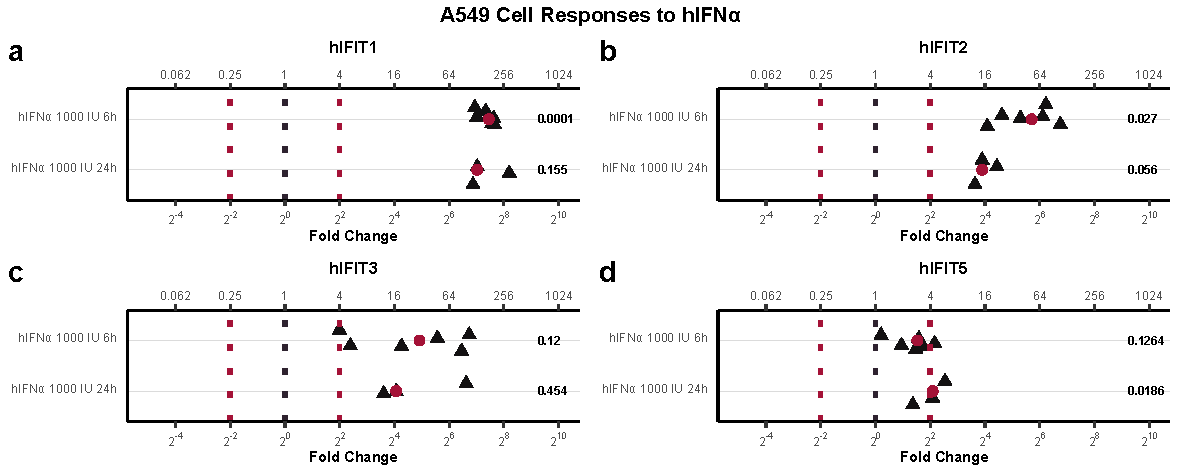
\includegraphics[width=1\linewidth]{06. Chapter 1/Figs/01. Induction/01. a549_treat_ifna.pdf}
    \caption[qPCR Analysis of A549 \textit{hIFIT} Response to hIFN\(\alpha\).]{\textbf{qPCR Analysis of A549 \textit{hIFIT} to hIFN\(\alpha\).} The relative abundance of (a) \textit{hIFIT1}, (b) \textit{hIFIT2}, (c) \textit{hIFIT3}, and (d) \textit{hIFIT5} genes, extracted from the A549 cell line, with response to human interferon alpha (IFN\(\alpha\)) at a concentration of 1000 IU per mL for a treatment duration of 6 or 24 hours. The shown values are relative to standardised mock values. The red circles signify median values. The black dotted line indicates mock expression, while the red dotted lines indicate biologically significant levels of induction. Numeric values signify the p-values compared to mock.}
    \label{A549 Response to hIFNa}
\end{figure}

The A549 cell line, derived from   lung carcinomatous tissue from a 58-year-old Caucasian male in 1972 is a well-established model of alveolar epithelial cells, routinely used for cancer to viral research alike (\cite{Lieber1976ACells}). We observe that after the stimulation of the A549 cell line with 1,000 IU/mL of hIFN\(\alpha\) for either 6 or 24 hours human \textit{IFIT1}, \textit{IFIT2}, and \textit{IFIT3} were induced drastically, especially \textit{IFIT1}, which was induced around 200-fold (Figure \ref{A549 Response to hIFNa}). The relative induction levels were identical between \textit{IFIT2} and \textit{IFIT3}. For all of these 3 genes, we can observe a decreased expression with longer incubation of IFN\(\alpha\), i.e. approximately half of the induction levels caused by 6-hour long incubation. Human \textit{IFIT5} shows minimal induction compared to the other \textit{IFITs} (3 and 4-fold for 6 and 24-hour long incubation respectively), which hovers around the mark of what is considered biologically significant induction, especially for ISGs, which are supposed not to be highly basally expressed. We can also observe a reverse trend of the time dependency of hIFN\(\alpha\)-induced expression. This suggests differential induction sensitivities between \textit{hIFIT1} (highly induced), \textit{hIFIT2} and \textit{hIFIT3} (medium induced) and \textit{hIFIT5} (low induced). All \textit{hIFIT} values had normal distributions and unequal variance other than \textit{hIFIT5}, which had normal distribution and normal variance.

\begin{figure}
    \centering
    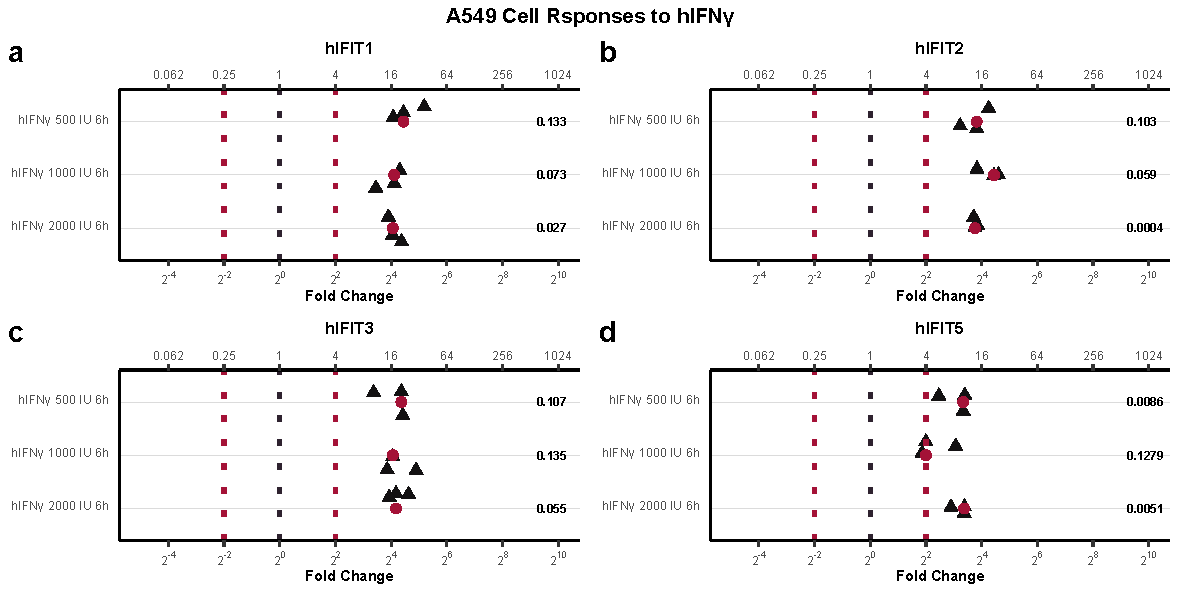
\includegraphics[width=1\linewidth]{06. Chapter 1/Figs/01. Induction/02. a549_treat_ifng.pdf}
    \caption[qPCR Analysis of A549 \textit{hIFIT} Response to hIFN\(\gamma\).]{\textbf{qPCR Analysis of A549 \textit{hIFIT} Response to hIFN\(\gamma\).} The relative abundance of (a) \textit{hIFIT1}, (b) \textit{hIFIT2}, (c) \textit{hIFIT3}, and (d) \textit{hIFIT5} genes, extracted from the A549 cell line, with response to human interferon-gamma (IFN\(\gamma\)) at concentrations of 500, 1000, and 2000 IU per mL for a treatment duration of 6 hours. The shown values are relative to standardised mock values. The red circles signify median values. The black dotted line indicates mock expression, while the red dotted lines indicate biologically significant levels of induction. Numeric values signify the p-values compared to mock.}
    \label{A549 Response to hIFNg}
\end{figure}

The response of human \textit{IFIT} genes to human IFN gamma can be seen in Figure \ref{A549 Response to hIFNg}. We can observe all \textit{IFITs} other than \textit{hIFIT5} responding equally to all concentrations tested i.e. 500, 1,000 and 2,000 IU/mL. Their response was concentration independent of a magnitude of around 15-fold. \textit{hIFIT5} response to very low concentration and very high concentrations was around 10-fold, while its transcript abundance increased only 4 times when treated with 1,000 IU/mL concentration. This suggests that the interferon-gamma component of the human \textit{IFIT} response is relatively equal for all of the \textit{IFIT} genes. This data, along with the data from hIFN\(\alpha\) induction also confirms that the A549 cell line is \textit{hIFIT} induction capable, which is great. All \textit{hIFIT} values had normal distributions and unequal variance other than \textit{hIFIT5}, which had normal distribution and normal variance.

\begin{figure}
    \centering
    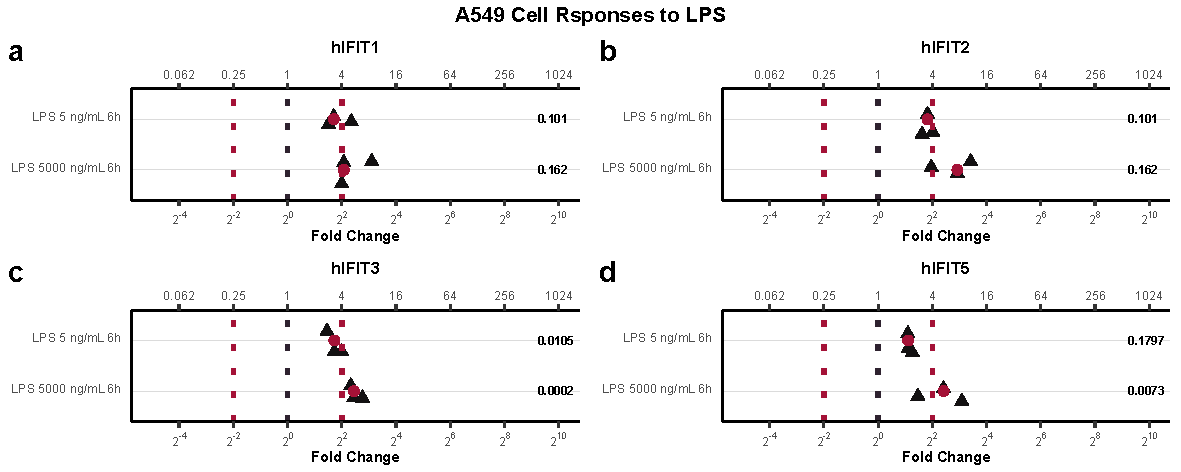
\includegraphics[width=1\linewidth]{06. Chapter 1/Figs/01. Induction/03. a549_treat_lps.pdf}
    \caption[qPCR Analysis of A549 \textit{hIFIT} Response to LPS.]{\textbf{qPCR Analysis of A549 \textit{hIFIT} Response to LPS.} The relative abundance of (a) \textit{hIFIT1}, (b) \textit{hIFIT2}, (c) \textit{hIFIT3}, and (d) \textit{hIFIT5} genes, extracted from the A549 cell line, with response to lipopolysaccharide (LPS) at concentrations of 5 and 5000 ng/mL for a treatment duration of 6 hours. The shown values are relative to standardised mock values. The red circles signify median values. The black dotted line indicates mock expression, while the red dotted lines indicate biologically significant levels of induction. Numeric values signify the p-values compared to mock.}
    \label{A549 Response to LPS}
\end{figure}

In order to assess the involvement of TLR4, a receptor also responsible for detecting RSV particles, A549 cells were incubated for 6 hours with low (5 ng/mL) and high (5,000 ng/mL) concentrations of bacterial LPS, its known activator. We can see that all \textit{IFITs} respond in a concentration dependant manner but the response is the lowest out of the different stimulants used. Low-concentration LPS incubation causes biologically insignificant induction of all \textit{hIFITs} of 2-fold for \textit{hIFIT5} and 3-fold for the other \textit{IFITs}. The high concentration on the other hand yields biologically significant induction levels of 4-8 fold induction. All \textit{hIFIT} values had normal distributions and unequal variance other than \textit{hIFIT3}, which had normal distribution and normal variance.

\begin{figure}
    \centering
    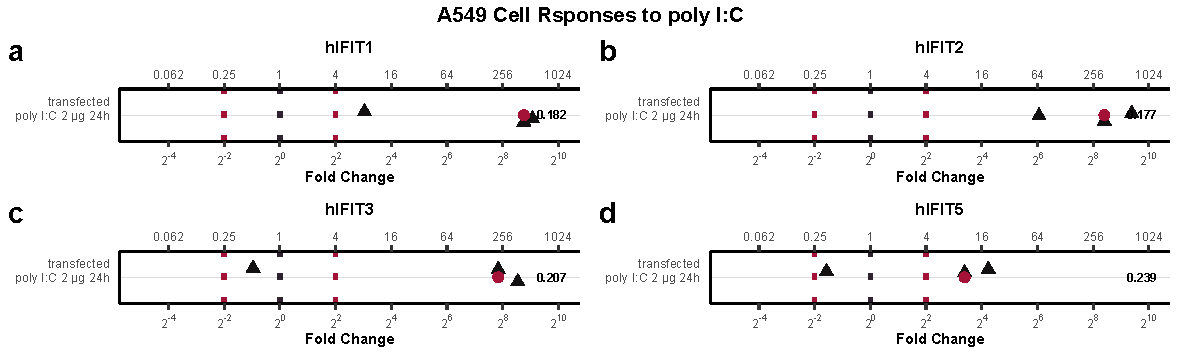
\includegraphics[width=1\linewidth]{06. Chapter 1/Figs/01. Induction/04. a549_treat_polyic.pdf}
    \caption[qPCR Analysis of A549 \textit{hIFIT} Response to Transfected poly I:C.]{\textbf{qPCR Analysis of A549 \textit{hIFIT} Response to Transfected poly I:C.} The relative abundance of (a) \textit{hIFIT1}, (b) \textit{hIFIT2}, (c) \textit{hIFIT3}, and (d) \textit{hIFIT5} genes, extracted from the A549 cell line. The cells were transfected with 2 \(\mu\)g of poly I:C for 24 hours. The shown values are relative to standardised mock values. The red circles signify median values. The black dotted line indicates mock expression, while the red dotted lines indicate biologically significant levels of induction. Numeric values signify the p-values compared to mock.}
    \label{A549 Response to poly I:C}
\end{figure}

When A549 cells were transfected with 2\(\mu\)g of poly I:C for 24 hours we were able to observe the biggest induction compared to the other inducers previously used (Figure \ref{A549 Response to poly I:C}). As with the other inducers, hIFIT1 induction is the greatest (circa 500-fold), followed by \textit{hIFIT2} and \textit{hIFIT3} with 300-fold and 200-fold responses respectively, with \textit{hIFIT5} trailing behind with the lowest response of only 10-fold. This again suggests that \textit{hIFIT5} seems to have differential transcriptomic regulation compared to the other genes of the \textit{IFIT} family. All \textit{hIFIT} values had normal distributions and unequal variance.

\begin{figure}
    \centering
    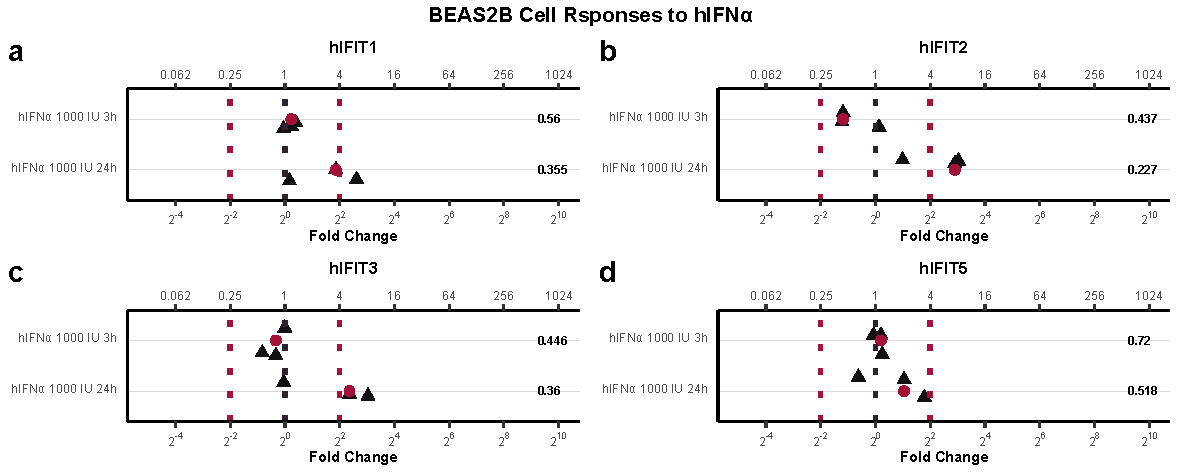
\includegraphics[width=1\linewidth]{06. Chapter 1/Figs/01. Induction/09. beas2b_ifna.pdf}
    \caption[qPCR Analysis of BEAS-2B \textit{hIFIT} Response to hIFN\(\alpha\).]{\textbf{qPCR Analysis of BEAS-2B \textit{hIFIT} Response to hIFN\(\alpha\).} The relative abundance of (a) \textit{hIFIT1}, (b) \textit{hIFIT2}, (c) \textit{hIFIT3}, and (d) \textit{hIFIT5} genes, extracted from the BEAS-2B cell line, with response to human interferon alpha (IFN\(\alpha\)) at a concentration of 1000 IU per mL for a treatment duration of 3 or 24 hours. The shown values are relative to standardised mock values. The red circles signify median values. The black dotted line indicates mock expression, while the red dotted lines indicate biologically significant levels of induction. Numeric values signify the p-values compared to mock.}
    \label{BEAS-2B responses to hIFNa}
\end{figure}

Lastly, we validated the human interferon alpha induction data in a more biologically relevant cell line, BEAS-2B. Established from bronchial epithelial biopsies from healthy samples, and later immortalised using the transfection of cyclin-dependent kinase 4 and human telomerase reverse transcriptase, these cells are an invaluable tool in the field of bronchial development and pathogenesis (\cite{Ramirez2004ImmortalizationOncoproteins}). After the treatment with human interferon alpha at concentrations of 1,000 IU/mL for 3 hours, we can see that this stimulation was not sufficient to induce the expression of any human \textit{IFIT} (Figure \ref{BEAS-2B responses to hIFNa}). However, when the cells were stimulated for 24 hours we can observe induction above biological significance for \textit{hIFIT1}, \textit{hIFIT2}, and \textit{hIFIT3}, with 4-fold, 8-fold, and 5-fold increase respectively. \textit{hIFIT5} shows only 2-fold median induction, which could be caused by the intrinsic variability of the assay. So as we observed with the A549 cell line, \textit{hIFIT5} behaves in discord with the other human \textit{IFITs}. All \textit{hIFIT} values had normal distributions and unequal variance.


\subsubsection{Human \textit{IFITs} Responses to Human RSV Infection} \label{Human \textit{IFITs} Responses to Human RSV}
After successfully confirming the \textit{IFIT} induction competency of  our workhorse cell line A549 as well as in the more physiologically relevant cell line BEAS-2B, we turn our attention to assessing the effect of human RSV infection on \textit{hIFIT} induction. To date, no studies have ever investigated this. Initially, we wanted to assess the effect of low, medium and high (0.1, 1, and 2 MOI respectively) infections as well as short and long-term infections (24 and 48 HPI respectively) on \textit{hIFIT} induction. My colleagues in the Viral Glycoproteins from the Pirbright Institute routinely perform hRSV infections of both A549 and BEAS-2B cell lines and thus the knowledge of what constitutes low and high MOI infection, as well as what short and long infection periods are widely known and available (I GUESS SOME CITATION HERE).  The virus was prepared and quantified as described in Section \ref{Virus Propagation and Production} and Section \ref{Virus Quantification by TCID50 Assay}. Briefly, infected cells were sonicated, cell debris was separated by centrifugation and virus-containing supernatant was gathered and titred. A549 cells were infected with the hRSV-containing supernatant at multiplicities of infection (MOI) of 0.1, 1,  and 2. Total mRNA was collected from the samples either 24 or 48 hours post-infection (HPI) and converted to complementary DNA, as described in Section \ref{RNA Extraction and cDNA Synthesis}. This was subsequently quantified by qPCR as described in Section \ref{Quantitative PCR} and the data analysed as described in Section \ref{Data Processing}. The responses of \textit{hIFITs} as a function of HPI and MOI can be seen in Figure \ref{A549 response to hRSV timepoints}, along with a plot quantifying human \textit{RSV N} mRNA as a control for viral replication. The relative quantification values of \textit{RSV N} has to be taken with a grain of salt as it is being compared to mock-infected samples that should have no \textit{RSV N} mRNA present. As a result, the actual relative values are dependent on the Ct values detected in the mock. 
 

\begin{figure}
    \centering
    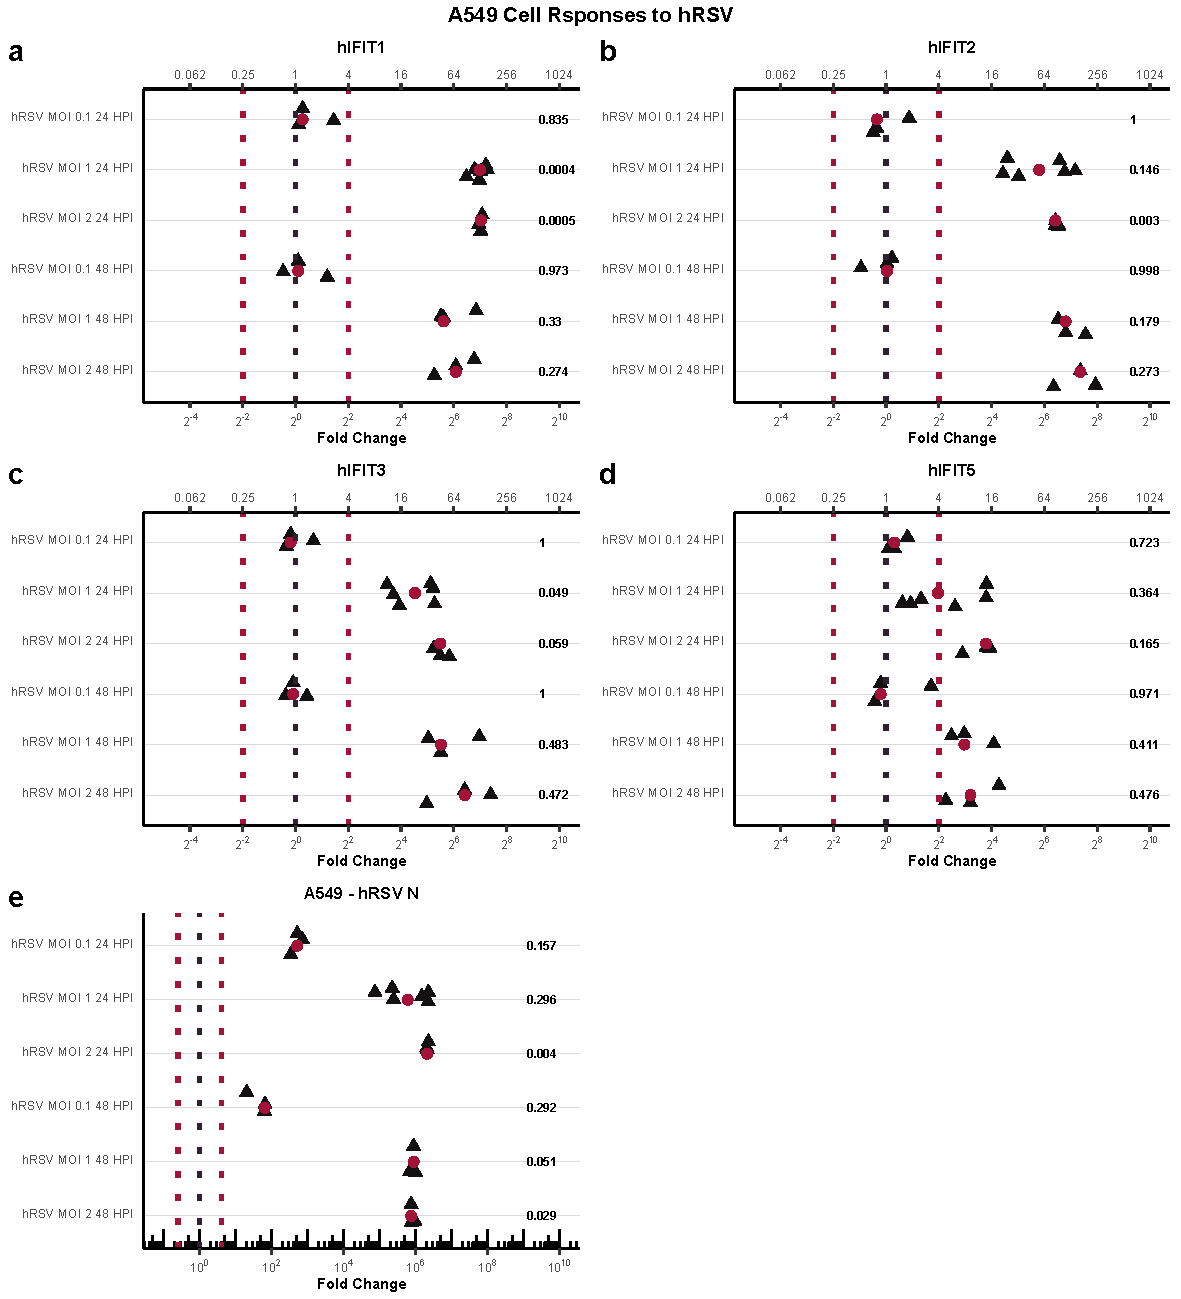
\includegraphics[width=1\linewidth]{06. Chapter 1/Figs/01. Induction/05. a549_hrsv_timepoints.pdf}
    \caption[A549 \textit{hIFIT} Response to hRSV as a Function of Time and MOI.]{\textbf{A549 \textit{hIFIT} Response to hRSV as a Function of Time and MOI.} The relative abundance of (a) \textit{hIFIT1}, (b) \textit{hIFIT2}, (c) \textit{hIFIT3}, (d) \textit{hIFIT5}, and (e) \textit{hRSV N} genes, extracted from A549 cell line following infection with human RSV at MOI of either 0.1, 1, or 2 for either 24 or 48 hours post-infection. The shown values are relative to standardised mock values. The red circles signify median values. The black dotted line indicates mock expression, while the red dotted lines indicate biologically significant levels of induction. Numeric values signify the p-values compared to mock.}
    \label{A549 response to hRSV timepoints}
\end{figure}


First of all, we can observe low MOI infection, although causing a productive infection as seen by \textit{hRSV N} mRNA relative quantification, did not yield any relative change of \textit{hIFIT} levels, suggesting that their induction is dependant not solely on the viral replication, but on the underlying magnitude of infection. In general, MOI 2 infection yields higher induction for all \textit{hIFITs}, although the magnitude is comparable with MOI 1 infections. \textit{hIFIT1} is induced the highest out of the other genes at 24 HPI, with both MOI 1 and 2 reaching 120-fold induction levels, while the induction magnitude diminishes slightly at 48 HPI, where infections at MOI 1 and 2 yield 50-fold and 80-fold median induction values. As seen previously in Section \ref{Human IFIT Responses to Known Activators of Innate Immune Response}, \textit{hIFIT2} and \textit{hIFIT3} display very similar trends of induction (with the only difference being \textit{hIFIT2} responses being 2 times the ones of \textit{hIFIT3}) for all the conditions tested here. In more detail, 24 HPI \textit{hIFIT2} gets induced 60-fold and 90-fold to the MOI of 1 and 2 respectively, while at 48 HPI the median induction magnitude increases to 100-fold and 120-fold respectively. This makes \textit{hIFIT2} the highest induced \textit{hIFIT} at 48 HPI. This also suggest that the induction dynamics of \textit{hIFIT1} differ from those of \textit{hIFIT2} and \textit{hIFIT3}. With regards to \textit{hIFIT5}, it displays the lowest, albeit still biologically significant induction for MOIs 1 and 2 for both time-points tested at median induction levels of 4 and 12 for 24 HPI MOIs 1 and 2 respectively, and 9 and 10 for 48 HPI MOIs 1 and 2 respectively. All datasets were of normal distribution and non-equal variance.


\begin{figure}
    \centering
    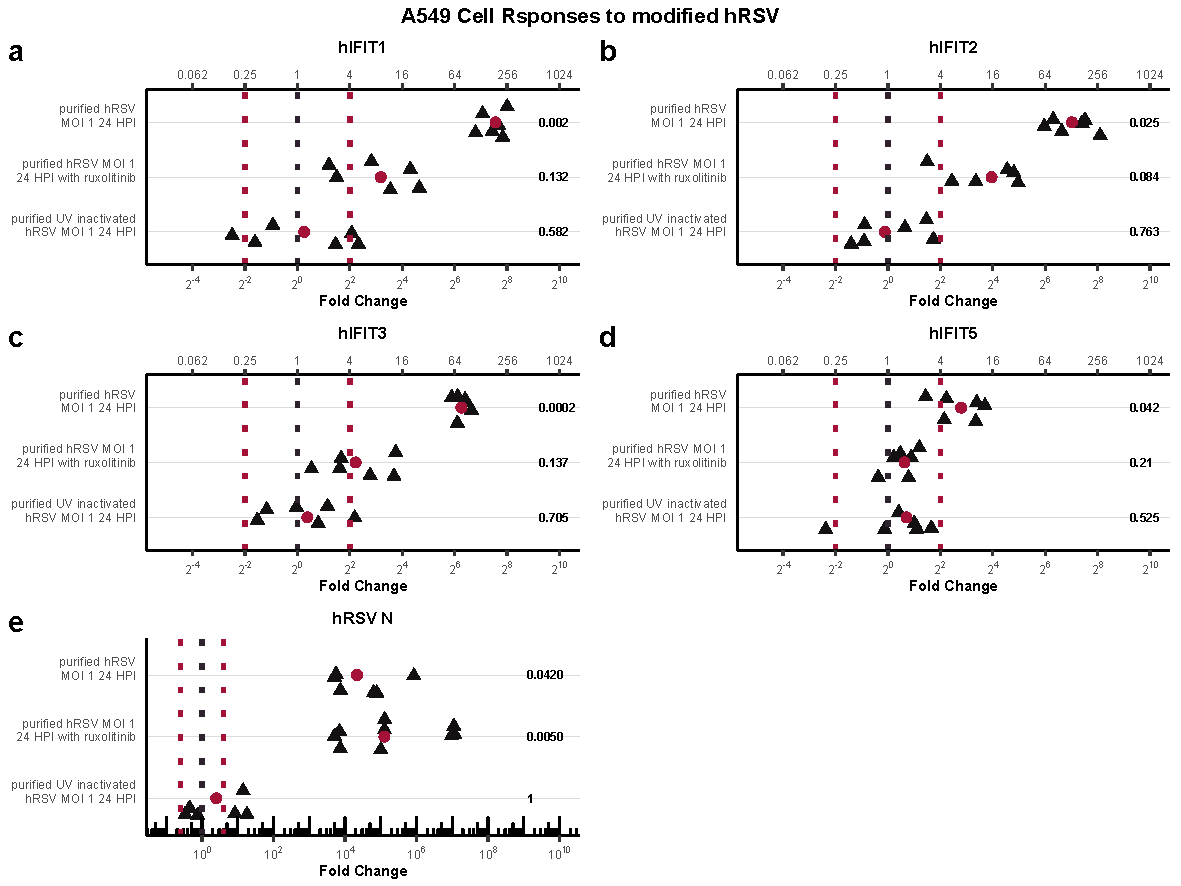
\includegraphics[width=1\linewidth]{06. Chapter 1/Figs/01. Induction/06. a549_hrsv_uv_roxo.pdf}
    \caption[The Effect of Ultra-Purification, UV-Inactivation and INFR Inhibition on \textit{hIFIT} Induction Following hRSV Infection in A549.]{\textbf{The Effect of Ultra-Purification, UV-Inactivation and INFR Inhibition on \textit{hIFIT} Induction Following hRSV Infection in A549.} The relative abundance of (a) \textit{hIFIT1}, (b) \textit{hIFIT2}, (c) \textit{hIFIT3}, (d) \textit{hIFIT5}, and (e) \textit{hRSV N} genes, extracted from A549 cell line following infection with ultra-purified hRSV at MOI 1 for 24 hours. The cells were either treated with the virus alone (first row), or with the virus and 5 nM of ruxolitinib (interferon receptor inhibitor) during the whole infection period (second row), or with UV-inactivated hRSV (last row). The shown values are relative to standardised mock values. The red circles signify median values. The black dotted line indicates mock expression, while the red dotted lines indicate biologically significant levels of induction. Numeric values signify the p-values compared to mock.}
    \label{The effect of ultra-purification, UV-inactivation and INFR inhibition on hIFIT induction following hRSV infection in A549}
\end{figure}

After confirming and concluding that human RSV infection indeed induces \textit{hIFIT} mRNA expression, we wanted to investigate the underlying induction principles. We wanted to investigate if the induction observed is indeed caused by human RSV detection and not by any other contaminants present in the virus prep such as cytokines, chemokines, and other stimulants. To do this, we created ultra-purified hRSV preps by ultra-centrifugation on a discontinuous sucrose cushion, as described in Section \ref{Virus Propagation and Production}. We also wanted to test if it is predominately the infected cells that have the \textit{hIFIT} expression increased as a defence mechanism to acute infection, or if the infected cells stimulate the \textit{hIFIT} expression in neighbouring cells as a prophylactic against the infection, or both. To test this, after the infection procedure, we incubated the cells with 5 nM of ruxolitinib, a well established small molecule JAK/STAT inhibitor, as is described in Section \ref{Viral Infections, UV-Inactivation and Ruxolitinib Treatment}. Based on the observations from Figure \ref{A549 response to hRSV timepoints} we used MOI of 1, 24 HPI to ensure sufficient \textit{hIFIT} induction, while decreasing the stress of the cells.  Lastly, we also hypothesised that viral replication is required for \textit{hIFIT} expression. To test this, some ultra-purified hRSV samples were UV-inactivated by a UV-cross-linker, as described in Section \ref{Viral Infections, UV-Inactivation and Ruxolitinib Treatment}.

The results of the experiment can be seen in Figure \ref{The effect of ultra-purification, UV-inactivation and INFR inhibition on hIFIT induction following hRSV infection in A549}. \textit{hRSV N} dataset was of normal distribution with equal variance, while all the other were of normal distribution and non-equal variance. We can see that although purified hRSV infection yielded lower induction compared to what was observed in Figure \ref{A549 response to hRSV timepoints} with regards to hRSV MOI 1 24 HPI infection (\(10^6\)-fold to \(10^{4.5}\)-fold), it induced all \textit{hIFITs}, even to higher mounts that what was seen with crude-extracted virus. In more detail, \textit{hIFIT1} was induced the highest at 180-fold (compared to 120-fold observed previously), closely followed by \textit{hIFIT2}, which median induction was at 180-fold (compared to 80-fold observed previously). \textit{hIFIT3} induction was 75-fold, double what was seen previously with crude extracted hRSV, while \textit{hIFIT5} median induction was 6-fold, a very comparable level to 4-fold that was observed previously. Regardless of the absolute magnitude of the relative values, this data suggest that the main driving force in hRSV presence and not contaminants in the viral prep. With regards to the effect of JAK/STAT inhibitor ruxolitinib, its presence diminished induction of all \textit{hIFITs}. \textit{hIFIT1}, \textit{hIFIT2}, and \textit{hIFIT3} maintained median induction values above the biologically significant threshold at 8, 10, and 5-fold respectively, while \textit{hIFIT5} showed only minimal median induction value of only 1.5-fold. We can also observe an order of magnitude more \textit{hRSV N} mRNA detection, suggesting that inhibiting interferon signalling is beneficial for the virus, which makes sense. Lastly, we assessed how a detection of non-replicative hRSV particles contribute to \textit{hIFIT} induction. UV-cross-linking of hRSV inhibited viral replication, as can be seen by the {hRSV N} mRNA quantification. This in fact prevented induction of all the \textit{hIFITs}, suggesting that TLR4 sensing of RSV particle is not sufficient to initiate signalling cascades that would lead to \textit{hIFIT} induction. All together, this data suggest that hRSV particles indeed drive the \textit{hIFIT} induction, however, they have to be replication competent. Additional essential aspect is the presence of functional interferon signalling cascades and the underlying paracrine interferon signalling initiated by infected cells in order to protect its neighbours.

\begin{figure}
    \centering
    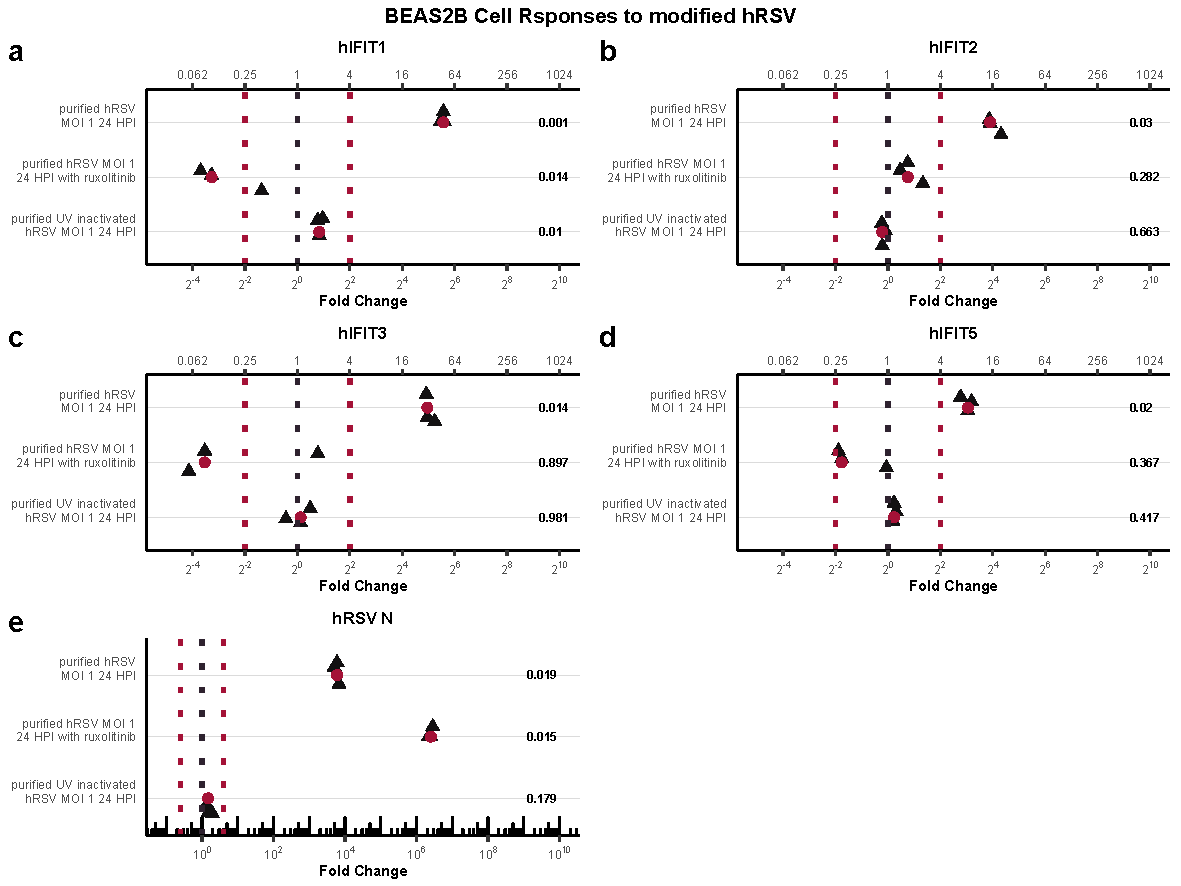
\includegraphics[width=1\linewidth]{06. Chapter 1/Figs/01. Induction/10. beas2b_hrsv.pdf}
    \caption[The Effect of Ultra-Purification, UV-Inactivation and INFR Inhibition on \textit{hIFIT} Induction Following hRSV Infection in BEAS-2B.]{\textbf{The Effect of Ultra-Purification, UV-Inactivation and INFR Inhibition on \textit{hIFIT} Induction Following hRSV Infection in BEAS-2B.} The relative abundance of (a) \textit{hIFIT1}, (b) \textit{hIFIT2}, (c) \textit{hIFIT3}, (d) \textit{hIFIT5} and (e) \textit{hRSV N} genes, extracted from BEAS-2B cell line following infection with ultra-purified hRSV at MOI 1 for 24 hours. The cells were either treated with the virus alone (first row), or with the virus and 5 nM of ruxolitinib (interferon receptor inhibitor) during the whole infection period (second row), or with UV-inactivated hRSV (last row). The shown values are relative to standardised mock values. The red circles signify median values. The black dotted line indicates mock expression, while the red dotted lines indicate biologically significant levels of induction. Numeric values signify the p-values compared to mock.}
    \label{The effect of ultra-purification, UV-inactivation and INFR inhibition on hIFIT induction following hRSV infection in BEAS-2B}
\end{figure}

Next we validated the findings using BEAS-2B cell line. We recreated the experiment from Figure \ref{The effect of ultra-purification, UV-inactivation and INFR inhibition on hIFIT induction following hRSV infection in A549} and the results can be seen in Figure \ref{The effect of ultra-purification, UV-inactivation and INFR inhibition on hIFIT induction following hRSV infection in BEAS-2B}. All datasets were of normal distribution and non-equal variance. All \textit{hIFITs} are induced to biologically significant levels by the infection of ultra-purified hRSV infection by 40, 15, 32, and 7-fold for \textit{hIFIT1}, \textit{hIFIT2}, \textit{hIFIT3}, and \textit{hIFIT5} respectively. These responses are also significantly higher than what was observed with human interferon alpha treatment (Figure \ref{BEAS-2B responses to hIFNa}). In line to what we have seen in A549 cell line, \textit{hIFIT1} is the highest induced, while \textit{hIFIT5} responds the worst to the infection. Interestingly, \textit{hIFIT3} median induction is higher than the one of \textit{hIFIT2}. When looking at the effect of ruxolitinib we can see that it prevented the induction of \textit{hIFIT2} and actually significantly decreased the relative levels of \textit{hIFIT1}, \textit{hIFIT3}, and \textit{hIFIT5} to the levels of \(2^{-3}\), \(2^{-3.5}\), and \(2^{-2}\) respectively. This suggest that not only is the interferon signalling required for \textit{hIFIT2} induction, it is vital for the maintenance  of basal \textit{hIFIT1}, \textit{hIFIT3}, and \textit{hIFIT5} levels in this cell line. Lastly, when the cells were infected with UV irradiated ultra-purified hRSV, none of the \textit{hIFITs} relative expression changed to biologically significant levels. This is in line to what we observed with A549 cell line. Taken together, we validate that replication competent viral particles are required for \textit{hIFIT} induction and while functional interferon receptor signalling cascades as also required, as we have seen in A549, in BEAS-2B they are necessary for maintaining the basal expression levels of \textit{hIFIT1}, \textit{hIFIT3}, and \textit{hIFIT5} mRNA levels.


\begin{figure}
    \centering
    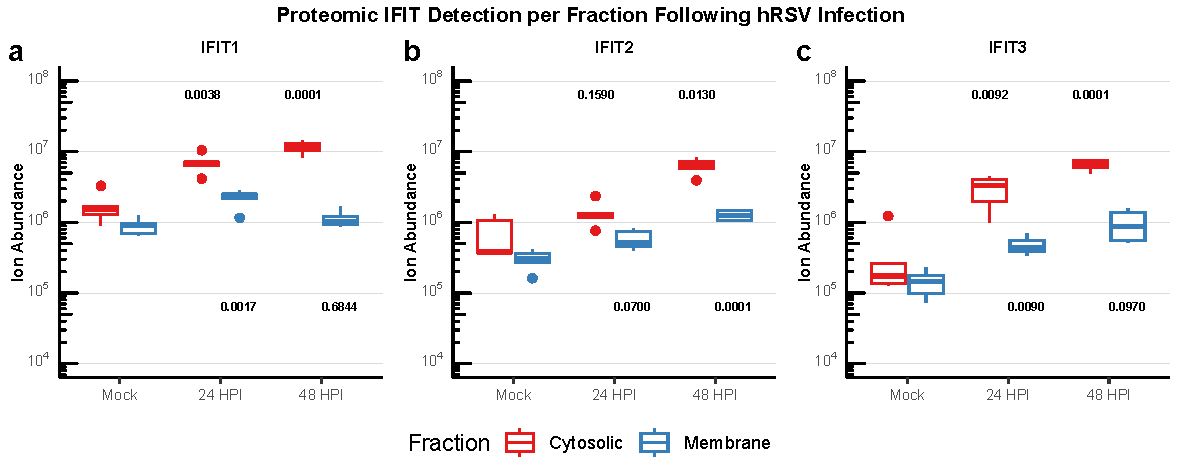
\includegraphics[width=1\linewidth]{06. Chapter 1/Figs/01. Induction/13. merged_proteomics.pdf}
    \caption[Human IFIT proteins detected per fraction.]{\textbf{Human IFIT proteins detected per fraction.} Analysis of summed peptide intensities of (a) hIFIT1, (b) hIFIT2, and (c) hIFIT3 detected per either cytosolic or membrane fractions of A549 cells which were either mock-infected, or infected with hRSV MOI 1 for either 24 or 48 hours.There were no hits for IFIT5. This data is from a proteomic study, published in \cite{Jobe2023ViralCondensates}. Samples are composed of biological quintuplicates. Numeric values signify the p-values compared to mock the respective mock, i.e. top numbers for cytosolic fraction, bottom for membrane fraction.}
    \label{Human IFIT proteomics.}
\end{figure}

To conclude the assessment of human IFIT responses to human RSV, I was kindly provided by a quantitative mass spectrometry dataset of human IFITs detected in either cytosolic or membrane fraction of either mock-infected or cells infected with human RSV at MOI 1, processed 24 or 48 HPI. This dataset was provided by Dr. Kelly and Dr. Jobe from the Pirbright Institute and its findings have now been published (\cite{Jobe2023ViralCondensates}). Quintuplicate of cytosolic and membrane fractions were isolated by in-gel digestion and analysed by label free quantitative mass spectrometry. Normalised and log transformed ion abundance data for hIFIT1, hIFIT2, and hIFIT3 can be seen in Figure \ref{Human IFIT proteomics.}. hIFIT1 cytoplasmic and hIFIT2 membrane datasets had normaldistributions and equal variances, while all the others displayed normal distributions with non-equal variances. Human IFIT5 did not yield any hits and thus was excluded from the analysis and we can conclude that its proteome is not drastically changed by hRSV infection, with is in line with our qPCR data. hIFIT1 is the most basally abundant, followed by hIFIT2 and hIFIT3. The basal abundance of hIFITs is around equal between the fractions. The infection at 24 HPI causes increased abundance of all hIFITs in all fraction, more specifically hIFIT1 increased 5x in cytosolic fraction and 1.3x in membrane fraction; hIFIT2 increased 4x in cytosolic and 2xin membrane fractions; and hIFIT3 increased relatively the most by 13.5x in cytosolic fraction and 3x in membrane fraction. The highest total abundance at 24 HPI was still hIFIT1. At 48 HPI we can observe further increase in abundance for all other than hIFIT1 in membrane fraction which decreased to mock levels. In more detail, hIFIT1 in cytosolic fraction increased further 2x; hIFIT2 increased further 5x in cytosolic and 4x in membrane fraction; and hIFIT3 further increased 3x in cytosolic fraction and 2.5x in membrane fraction. These data together validate our qPCR results seen in Figure \ref{A549 response to hRSV timepoints} and Figure \ref{The effect of ultra-purification, UV-inactivation and INFR inhibition on hIFIT induction following hRSV infection in A549} and highlight the differential spatio-temporal expression dynamics of human IFITs.


\subsubsection{Human \textit{IFITs} Responses to bRSV Infection} \label{Human IFITs Responses to bRSV}
We were interested knowing if there is cross-species protection between hRSV and bRSV, with regards to cell infectivity and \textit{hIFIT} induction. We had an arsenal of several bRSV viruses including the wild-type (WT) along with a panel of mutant viruses with deletions of small-hydrophobic (SH) protein, non-structural (NS) protein 1 or 2 or both (see Table \ref{Outline of Viruses Used table}). As described in INTRODUCTION these proteins are responsible for STUFF FROM INTRODUCTION. The viruses were prepared and quantified as described in Section \ref{Virus Propagation and Production} and Section \ref{Virus Quantification by TCID50 Assay}. Briefly, infected cells were sonicated, cell debris was separated by centrifugation and virus-containing supernatant was gathered and titred. It is to be noted that due to the lack of the anti-antiviral proteins meant the virus preparation of \(Delta\)NS viruses had orders of magnitude lower titre than the other viruses. Regardless, A549 cells were initially infected with the WT and \(Delta\)SH bRSV-containing supernatant at MOI of 1. Total mRNA was collected from the samples 24 HPI and converted to complementary DNA, as described in Section \ref{RNA Extraction and cDNA Synthesis}. This was subsequently quantified by qPCR as described in Section \ref{Quantitative PCR} and the data analysed as described in Section \ref{Data Processing}. The responses of \textit{hIFITs} as a function of HPI and MOI can be seen in Figure \ref{Responses of A549 to bRSV WT and dSH.}, along with a plot quantifying bovine \textit{RSV N} mRNA as a control for viral replication.

\begin{figure}
    \centering
    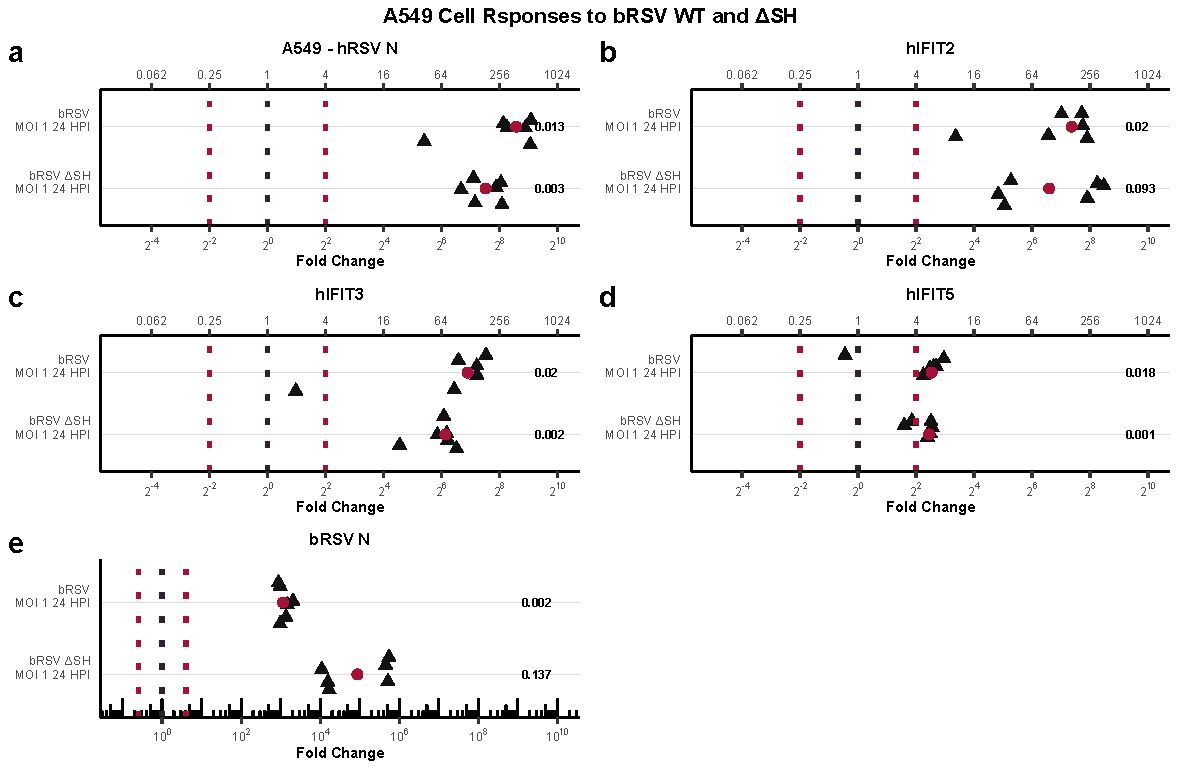
\includegraphics[width=1\linewidth]{06. Chapter 1/Figs/01. Induction/07. a549_brsv_moi1.pdf}
    \caption[A549 \textit{hIFIT} Response to WT and \(\Delta\)SH bRSV Infection.]{\textbf{A549 \textit{hIFIT} Response to WT and \(\Delta\)SH bRSV Infection.} The relative abundance of (a) \textit{hIFIT1}, (b) \textit{hIFIT2}, (c) \textit{hIFIT3}, (d) \textit{hIFIT5} and (e) \textit{bRSV N} genes, extracted from A549 cell line following infection with WT or \(\Delta\)SH bRSV at MOI 1, 24 HPI.  The shown values are relative to standardised mock values. The red circles signify median values. The black dotted line indicates mock expression, while the red dotted lines indicate biologically significant levels of induction. Numeric values signify the p-values compared to mock.}
    \label{Responses of A549 to bRSV WT and dSH.}
\end{figure}

We can see that both bRSV WT and bRSV \(\Delta\)SH were successfully replicating in the A549 cell line and this in fact both induced all \textit{hIFITs} to biologically significant levels. Interestingly, although bRSV \(\Delta\)SH \textit{N} relative mRNA levels were two orders of magnitude higher than the ones of WT bRSV, the detected indution magnitudes of \textit{hIFITs} were in general lower compared to the ones caused by bRSV WT infection. This is counterintuitive as the lack of SH protein should make the virus less infectious and thus show worse replication competency, while it should allow higher \textit{ISG} induction as there is less antagonism of the activation cascades present. Regardless, looking at the \textit{hIFITs} in more detail, \textit{hIFIT1} median induction by bRSV WT and \(\Delta\)SH infection was 400-fold and 150-fold respectively, which were again the highest induction magnitudes detected out of all \textit{hIFIT} response. On the other side of the spectrum is \textit{hIFIT5} with the median induction of 6-fold for both viruses, which are the lowest induction values and are consistent with what we observed so far throught the study. \textit{hIFIT2} was induced 180-fold and 80-fold by the WT and \(\Delta\)SH, while \textit{hIFIT3} was induced 128 and 70 fold respectively. Intriguingly, when compared to crude-extracted hRSV MOI 1 24 HPI from Figure \ref{A549 response to hRSV timepoints} we can see that although \textit{bRSV N} median relative abundances were two and one orders of magnitude lower for bRSV WT and \(\Delta\)SH respectively compared to \textit{hRSV N} but regardless, they caused greater induction of all \textit{hIFITs}. This suggest that bRSV is potentiated in human cells, probably due to the lack of species-specific inhibition, and this potentiation in turn causes higher \textit{hIFIT} induction as a response.

\begin{figure}
    \centering
    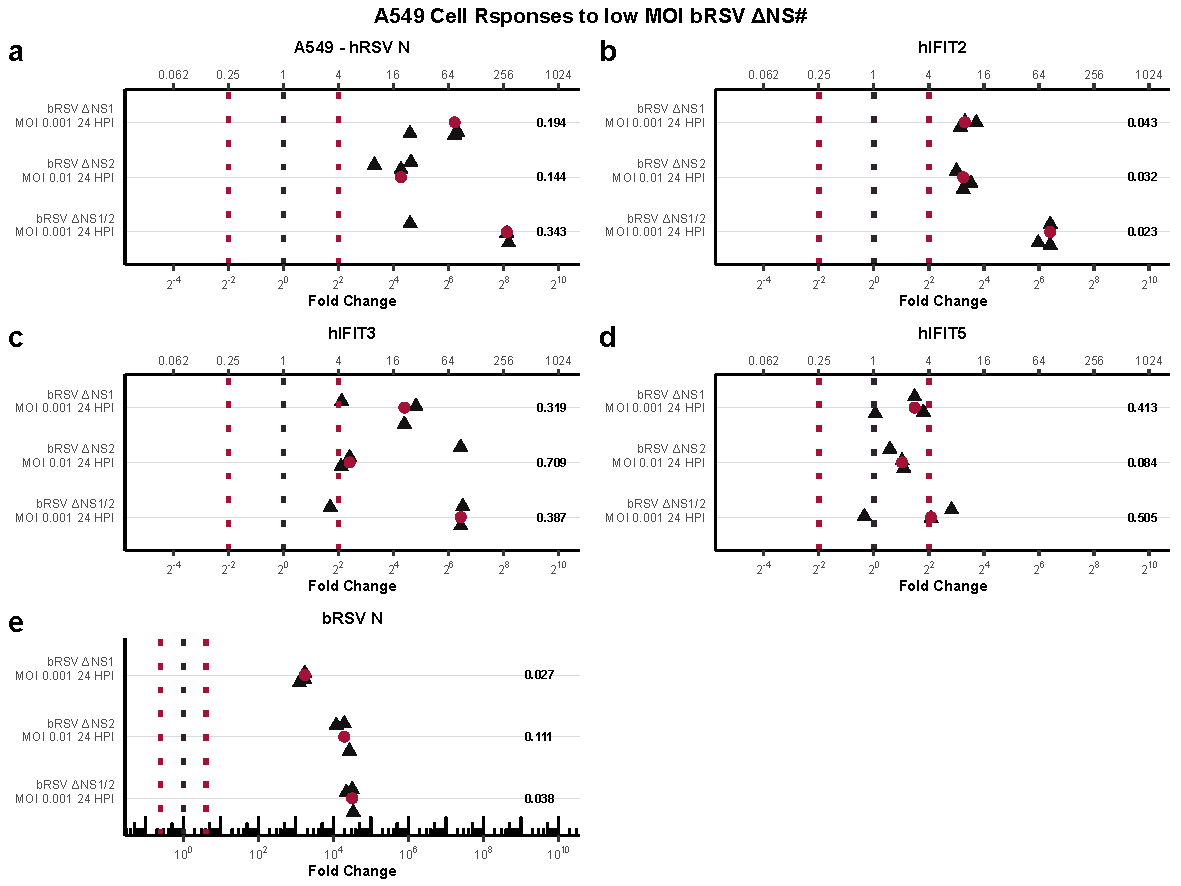
\includegraphics[width=1\linewidth]{06. Chapter 1/Figs/01. Induction/08. a549_brsv_dns.pdf}
    \caption[A549 \textit{hIFIT} Response to Low MOI \(\Delta\)NSs bRSV Infection.]{\textbf{A549 \textit{hIFIT} Response to Low MOI \(\Delta\)NSs bRSV Infection.} The relative abundance of (a) \textit{hIFIT1}, (b) \textit{hIFIT2}, (c) \textit{hIFIT3}, (d) \textit{hIFIT5} and (e) \textit{bRSV N} genes, extracted 24 HPI from A549 cell line following infection with bRSV \(\Delta\)NS1, \(\Delta\)NS2, and \(\Delta\)NS1/2 at MOIs of 0.001, 0.01, and 0.001 respectively. The shown values are relative to standardised mock values. The red circles signify median values. The black dotted line indicates mock expression, while the red dotted lines indicate biologically significant levels of induction. Numeric values signify the p-values compared to mock.}
    \label{Responses of A549 to bRSV dNSs.}
\end{figure}

Next, we investigated the effect of the rest of the mutant bRSV viruses, namely \(\Delta\)NS1, \(\Delta\)NS2, and a double knock-out \(\Delta\)NS1/2. As mentioned above, we had trouble achieving high titres using the crude-extraction methodology and thus the MOIs used are lower than what was conducted with WT and \(\Delta\)SH bRSV, more precisely 0.001 for \(\Delta\)NS1 and \(\Delta\)NS1/2, and 0.01 for \(\Delta\)NS2 bRSV. Total mRNA was extracted 24 hours post infection. In Figure \ref{Responses of A549 to bRSV dNSs.} we can see that all 3 viruses were able to successfully replicate, despite the low MOI. The replication magnitude mimics what was seen in Figure \ref{Responses of A549 to bRSV WT and dSH.} where \(\Delta\)NS1 \textit{bRSV N} mRNA levels were comparable to the wild-type infection and \(\Delta\)NS2 and \(\Delta\)NS1/2 levels were comparable to \(\Delta\)SH bRSV infection, although slightly lower. We can also observe mixed responses of \textit{hIFITs}, albeit all of them upregulation. \textit{hIFIT1} again was upregulated the highest, 70-fold, 20-fold and 300-fold to \(\Delta\)NS1, \(\Delta\)NS2, and \(\Delta\)NS1/2 respectively. \textit{hIFIT2} induction levels were almost identical for \(\Delta\)NS1 and \(\Delta\)NS2 viruses at around 8-fold despite the difference in MOI. \(\Delta\)NS1/2 bRSV infection induced it the highest, 70-fold. For \textit{hIFIT3} we can observe different induction dynamics. While \(\Delta\)NS1 infection induced it to higher levels that what we observed in \textit{hIFIT2} (20-fold), \(\Delta\)NS2 yielded barely biologically significant induction (4-fold), while virus lacking both non structural proteins induced \textit{hIFIT3} to equal levels as was observed with \textit{hIFIT2} (70-fold). Although we can see similar upregulation trends with \textit{hIFIT5} to what was observed with other \textit{hIFITs}, meaning \(\Delta\)NS1 causes medium induction, \(\Delta\)NS2 causes low induction, and \(\Delta\)NS1/2 causing high inducion, only the latter can be considered biologicaly significant (4-fold). Yet again, compared to the results with low MOI infection with hRSV (Figure \ref{A549 response to hRSV timepoints}), bRSV seems to be more replication competent, as seen by the relative \textit{bRSV N} mRNA levels, and a more potent \textit{hIFIT} inducer, as low MOI hRSV infection did not yield any induction what so ever. This data also highlights that NS1 negatively regulates \textit{hIFIT} induction more compared NS2, and a lack of both proteins seems to have a synergistic effect on \textit{hIFIT} induction.


\begin{figure}
    \centering
    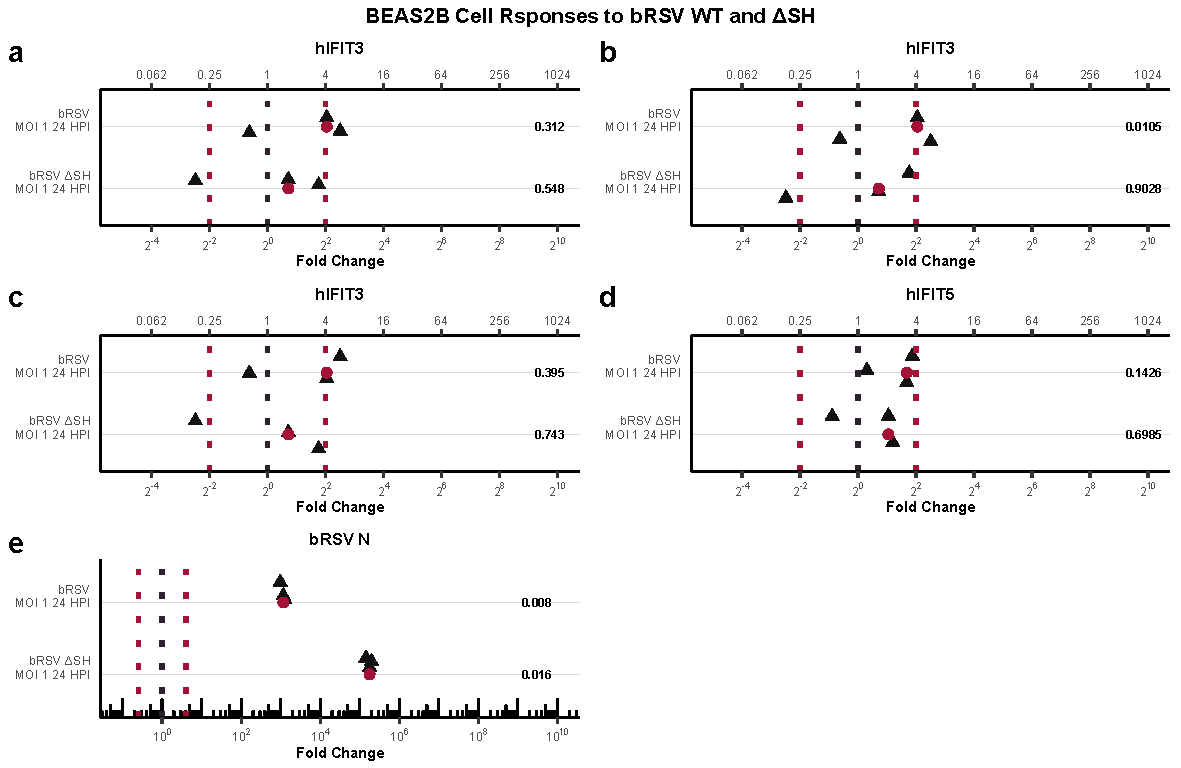
\includegraphics[width=1\linewidth]{06. Chapter 1/Figs/01. Induction/11. beas2b_brsv_moi1.pdf}
    \caption[BEAS-2B \textit{hIFIT} Response to WT and \(\Delta\)SH bRSV Infection.]{\textbf{BEAS-2B \textit{hIFIT} Response to WT and \(\Delta\)SH bRSV Infection.} The relative abundance of (a) \textit{hIFIT1}, (b) \textit{hIFIT2}, (c) \textit{hIFIT3}, (d) \textit{hIFIT5} and (e) \textit{bRSV N} genes, extracted from BEAS-2B cell line following infection with WT or \(\Delta\)SH bRSV at MOI 1, 24 HPI.  The shown values are relative to standardised mock values. The red circles signify median values. The black dotted line indicates mock expression, while the red dotted lines indicate biologically significant levels of induction. Numeric values signify the p-values compared to mock.}
    \label{BEAS-2B responses to bRSV WT and dSH.}
\end{figure}


Lastly we wanted to validate these results in BEAS-2B cell line. The experimental setup was identical to what was described above during the investigation of A549 \textit{hIFIT} responses to bRSV infection. Figure \ref{BEAS-2B responses to bRSV WT and dSH.} shows the induction levels caused by infection at MOI 1, 24 HPI with WT and \(\Delta\)SH bSRV. We can see, based on the median relative \textit{bRSV N} mRNA levels, that the viruses are capable of infecting BEAS-2B and are replicating approximately to the levels of what we observed in A549 cell line. We can also observe that the general trend from A549 one experiment is present, meaning \textit{hIFITs} are being positively induced, and more by the WT bRSV infection than the (\Delta\)SH one, with the difference being magnitude of these inductions. In more detail, the induction of all \textit{hIFITs} seems to be similar, barely biologically significant by WT infection (4-fold), and very weak by (\Delta\)SH infection (>2-fold). \textit{hIFIT5} is induced just below biological significance by WT bRSV and at the same level as the other \textit{hIFITs} by the mutant virus. So interestingly the \textit{hIFIT} induction seems to be cell line and stimulus specific.


\begin{figure}
    \centering
    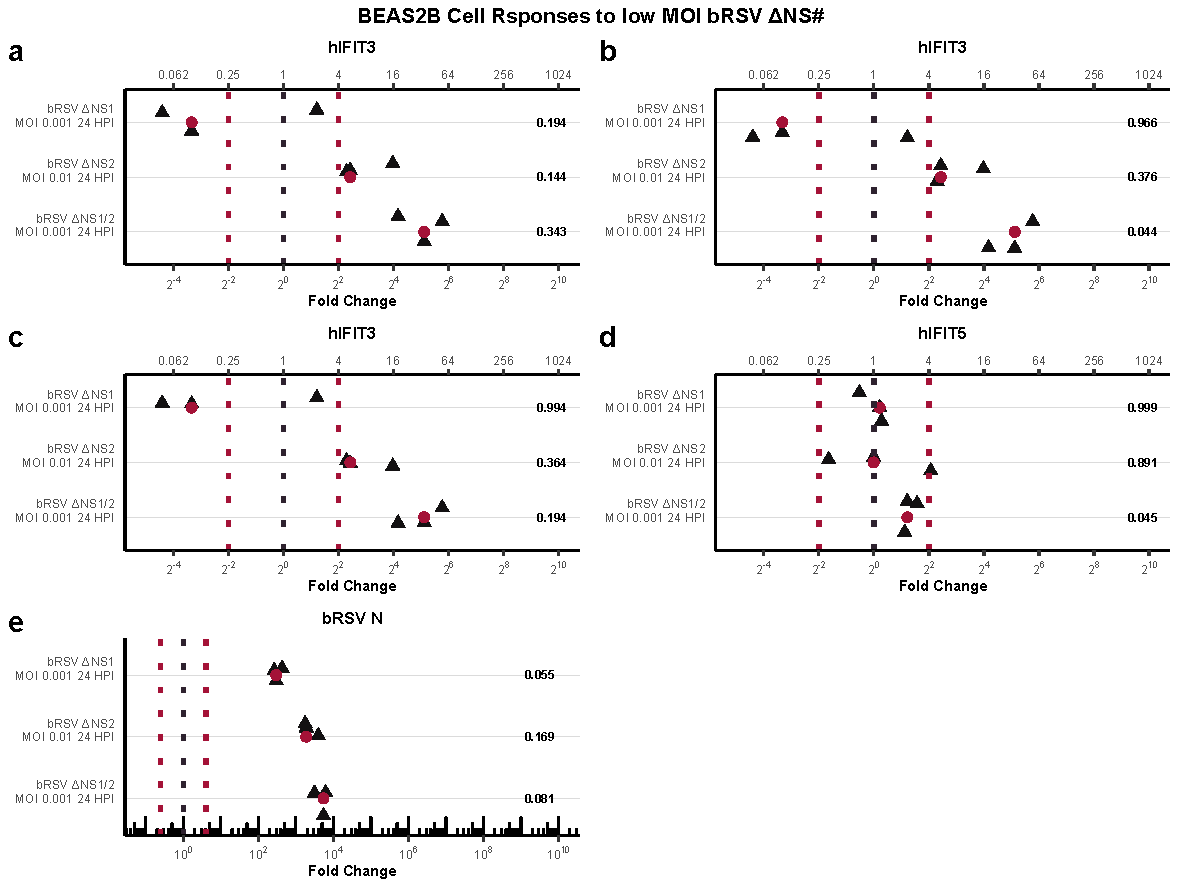
\includegraphics[width=1\linewidth]{06. Chapter 1/Figs/01. Induction/12. beas2b_brsv_dns.pdf}
    \caption[BEAS-2B \textit{hIFIT} Response to Low MOI \(\Delta\)NSs bRSV Infection.]{\textbf{BEAS-2B \textit{hIFIT} Response to Low MOI \(\Delta\)NSs bRSV Infection.} The relative abundance of (a) \textit{hIFIT1}, (b) \textit{hIFIT2}, (c) \textit{hIFIT3}, (d) \textit{hIFIT5} and (e) \textit{bRSV N} genes, extracted 24 HPI from BEAS-2B cell line following infection with bRSV \(\Delta\)NS1, \(\Delta\)NS2, and \(\Delta\)NS1/2 at MOIs of 0.001, 0.01, and 0.001 respectively. The shown values are relative to standardised mock values. The red circles signify median values. The black dotted line indicates mock expression, while the red dotted lines indicate biologically significant levels of induction. Numeric values signify the p-values compared to mock.}
    \label{BEAS-2B responses to bRSV dNSs.}
\end{figure}


Furthermore we validated the \(\Delta\)NSs infection data from A549 (Figure \ref{Responses of A549 to bRSV dNSs.}) using the same experimental setup as was described prevously. As we can see in Figure \ref{BEAS-2B responses to bRSV dNSs.}, the induction behaviour again differs from what we observed with A549 cell line. Based on \textit{bRSV N} mRNA levels, we can see that the mutant viruses were able to replicate, although the asolute relative values are one order of magnitude lower to what was observed with A549 cell line. \textit{hIFIT5} does not respond to the infection with \(\Delta\)NS1 and \(\Delta\)NS2 bRSv and positively but biologically significantly responds to \(\Delta\)NS1/2 virus. \textit{hIFIT1}, \textit{hIFIT2}, and \textit{hIFIT3} display very similar induction profile to the stimulant. More specificaly, \(\Delta\)NS1 infection downregulated all by \(2^{-3}\)-fold, while \(\Delta\)NS2 infection caused just biologically significant induction (4-fold), and the double mutant \(\Delta\)NS1/2 caused median induction of 32-fold. This data suggest NS1 protein being \textit{hIFIT} inductive, while the presence NS2 negatively influencing \textit{hIFIT} expression. This is in reverse to what we observed with A549. A lack of both non structural proteins seems to have synergisticly positive effect on \textit{hIFIT} induction, like we observed with the A549 cell line.

\subsubsection*{Summary} \label{Summary-human-induction}
Interestingly, the maximal induction of \textit{hIFIT5} observed in this study seems to be 10-16 fold, a order of magnitude lower of what is observed for the other \textit{hIFIT}.

\section{Conclusions} \label{sec:Conclusions Chapter 1}
Our experiments reveal the induction of human \textit{IFITs} in both A549 and BEAS2B cell lines, albeit with a more moderate response observed in BEAS2B. The induction trends are summarised in Table \ref{tab:Summary of Human IFIT Responses to Activators of Innate Immune Response.}. Further literature research uncovered that the BEAS2B cell line maintains higher basal expression of interferon-stimulated genes, providing a potential explanation for our observations \cite{Seng2014HighResistance}. Notably, both cell lines exhibit a time-dependent response to IFN$\upalpha$ stimulation in an inverse manner, indicating that \textit{hIFITs} are acute responders to IFN$\upalpha$ treatment. Interestingly, the varying induction magnitudes of \textit{IFITs} between the cell lines reveals that while \textit{IFIT5} shows the lowest induction levels in both cell lines, A549 has \textit{IFIT1} as the highest-induced IFIT, contrasting with BEAS2B, where \textit{IFIT2} was induced to the highest level. Additional A549 experiments demonstrate that LPS incubation stimulates \textit{IFIT} induction, but the magnitude, especially in comparison to other stimulants, appears biologically insignificant. Remarkably, IFN$\upgamma$ consistently elicits \textit{IFIT} induction in a concentration-independent manner, manifesting a uniform induction magnitude across various \textit{IFITs}—a characteristic not observed with other stimulants. Initially, these results were surprising, given our assumption that IFN$\upgamma$-mediated signalling was pertinent only to myeloid cell lines, a classification the A549 cell line does not fall under. However, published evidence on IFN$\upgamma$ receptor expression more broadly across cell types \cite{Ivashkiv2018IFN:Immunotherapy} and, more specifically, transcriptomic data in the A549 cell line reported in the Human Protein Atlas \cite{Uhlen2015Tissue-basedProteome}, corroborate the presence of IFN$\upgamma$ receptor expression in A549 cells. Moreover, transfected poly I:C induces \textit{IFITs} to levels surpassing those elicited by other tested innate immune system stimulants.

\begin{table}
    \centering
    \begin{tabular}{lllll}
    \hline
        \textbf{Cell Line} & \textbf{IFIT} & \textbf{Treatment} & \textbf{Figure} & \textbf{Trend} \\ \hline
        A549 & IFIT1 & hIFN$\upalpha$ 1000 IU 6h & Figure 3.1 & \(\uparrow\)\(\uparrow\) \\ 
        A549 & IFIT1 & hIFN$\upalpha$ 1000 IU 24h & Figure 3.1 & \(\uparrow\)\(\uparrow\) \\ 
        A549 & IFIT1 & hIFN$\upgamma$ 500 IU 6h & Figure 3.2 & \(\uparrow\) \\ 
        A549 & IFIT1 & hIFN$\upgamma$ 1000 IU 6h & Figure 3.2 & \(\uparrow\) \\ 
        A549 & IFIT1 & hIFN$\upgamma$ 2000 IU 6h & Figure 3.2 & \(\uparrow\) \\ 
        A549 & IFIT1 & LPS 5 ng/mL 6h & Figure 3.3 & \(\nearrow\) \\ 
        A549 & IFIT1 & LPS 5000 ng/mL 6h & Figure 3.3 & \(\nearrow\) \\ 
        A549 & IFIT1 & poly I:C 2 µg 24h & Figure 3.4 & \(\uparrow\)\(\uparrow\)\(\uparrow\) \\ 
        BEAS2B & IFIT1 & hIFN$\upalpha$ 1000 IU 3h & Figure 3.5 & \(\rightarrow\) \\ 
        BEAS2B & IFIT1 & hIFN$\upalpha$ 1000 IU 24h & Figure 3.5 & \(\nearrow\) \\ 
        A549 & IFIT2 & hIFN$\upalpha$ 1000 IU 6h & Figure 3.1 & \(\uparrow\) \\ 
        A549 & IFIT2 & hIFN$\upalpha$ 1000 IU 24h & Figure 3.1 & \(\uparrow\) \\ 
        A549 & IFIT2 & hIFN$\upgamma$ 500 IU 6h & Figure 3.2 & \(\uparrow\) \\ 
        A549 & IFIT2 & hIFN$\upgamma$ 1000 IU 6h & Figure 3.2 & \(\uparrow\) \\ 
        A549 & IFIT2 & hIFN$\upgamma$ 2000 IU 6h & Figure 3.2 & \(\uparrow\) \\ 
        A549 & IFIT2 & LPS 5 ng/mL 6h & Figure 3.3 & \(\nearrow\) \\ 
        A549 & IFIT2 & LPS 5000 ng/mL 6h & Figure 3.3 & \(\uparrow\) \\ 
        A549 & IFIT2 & poly I:C 2 µg 24h & Figure 3.4 & \(\uparrow\)\(\uparrow\)\(\uparrow\) \\ 
        BEAS2B & IFIT2 & hIFN$\upalpha$ 1000 IU 3h & Figure 3.5 & \(\searrow\) \\ 
        BEAS2B & IFIT2 & hIFN$\upalpha$ 1000 IU 24h & Figure 3.5 & \(\uparrow\) \\ 
        A549 & IFIT3 & hIFN$\upalpha$ 1000 IU 6h & Figure 3.1 & \(\uparrow\) \\ 
        A549 & IFIT3 & hIFN$\upalpha$ 1000 IU 24h & Figure 3.1 & \(\uparrow\) \\ 
        A549 & IFIT3 & hIFN$\upgamma$ 500 IU 6h & Figure 3.2 & \(\uparrow\) \\ 
        A549 & IFIT3 & hIFN$\upgamma$ 1000 IU 6h & Figure 3.2 & \(\uparrow\) \\ 
        A549 & IFIT3 & hIFN$\upgamma$ 2000 IU 6h & Figure 3.2 & \(\uparrow\) \\ 
        A549 & IFIT3 & LPS 5 ng/mL 6h & Figure 3.3 & \(\nearrow\) \\ 
        A549 & IFIT3 & LPS 5000 ng/mL 6h & Figure 3.3 & \(\uparrow\) \\ 
        A549 & IFIT3 & poly I:C 2 µg 24h & Figure 3.4 & \(\uparrow\)\(\uparrow\) \\ 
        BEAS2B & IFIT3 & hIFN$\upalpha$ 1000 IU 3h & Figure 3.5 & \(\rightarrow\) \\ 
        BEAS2B & IFIT3 & hIFN$\upalpha$ 1000 IU 24h & Figure 3.5 & \(\uparrow\) \\ 
        A549 & IFIT5 & hIFN$\upalpha$ 1000 IU 6h & Figure 3.1 & \(\nearrow\) \\ 
        A549 & IFIT5 & hIFN$\upalpha$ 1000 IU 24h & Figure 3.1 & \(\nearrow\) \\ 
        A549 & IFIT5 & hIFN$\upgamma$ 500 IU 6h & Figure 3.2 & \(\uparrow\) \\ 
        A549 & IFIT5 & hIFN$\upgamma$ 1000 IU 6h & Figure 3.2 & \(\nearrow\) \\ 
        A549 & IFIT5 & hIFN$\upgamma$ 2000 IU 6h & Figure 3.2 & \(\uparrow\) \\ 
        A549 & IFIT5 & LPS 5 ng/mL 6h & Figure 3.3 & \(\nearrow\) \\ 
        A549 & IFIT5 & LPS 5000 ng/mL 6h & Figure 3.3 & \(\uparrow\) \\ 
        A549 & IFIT5 & poly I:C 2 µg 24h & Figure 3.4 & \(\uparrow\) \\ 
        BEAS2B & IFIT5 & hIFN$\upalpha$ 1000 IU 3h & Figure 3.5 & \(\rightarrow\) \\ 
        BEAS2B & IFIT5 & hIFN$\upalpha$ 1000 IU 24h & Figure 3.5 & \(\nearrow\) \\ \hline
    \end{tabular}
    \caption[Summary of Human \textit{IFIT} Responses to Activators of Innate Immune Response.]{\textbf{Summary of Human \textit{IFIT} Responses to Activators of Innate Immune Response.} Trend arrows indicate abundance relative to mock-treated values: strong downregulation ($\downarrow$, 0.062-0.25); mild downregulation ($\searrow$, 0.25-0.5); no difference ($\rightarrow$, 0.5-1.5); mild upregulation ($\nearrow$, 1.5-4); moderate upregulation ($\uparrow$, 4-64); strong upregulation ($\uparrow\uparrow$, 64-258); very strong upregulation ($\uparrow\uparrow\uparrow$, 258-1024).}
    \label{tab:Summary of Human IFIT Responses to Activators of Innate Immune Response.}
\end{table}

Further, we confirmed that high MOI hRSV infection, but not low MOI infection, induces \textit{hIFIT} expression. The summary of all human \textit{IFIT} responses to hRSV infection can be seen in Table \ref{tab:Summary of Human IFIT Responses to hRSV Infection.}. We observed a concentration and time-dependent effect, which was maintained for at least 48 HPI, for all \textit{hIFITs} but \textit{hIFIT1}, which nevertheless showed the most robust induction out of all the genes tested. We confirmed that this induction isn't due to cellular contaminants from the viral preparation step, as infecting cells with purified virus induced similar patterns of gene expression. In A549, this induction was greatly diminished following pharmacological blockage of the interferon receptor, and completely abolished by UV-inactivation of hRSV, indicating the necessity of RSV replication for the initial \textit{IFIT} induction and functional interferon signalling for a robust \textit{IFIT} response. Most likely infected cells initiate an innate immune response, which also induces \textit{IFIT} locally and results in interferon production. This is then sensed by surrounding cells by paracrine interferon signalling, which in turn prophylactically induces \textit{IFIT} in those cells. This data was mirrored in the BEAS2B cell line, with minor discrepancies in the overall magnitude of \textit{IFIT} induction—aligning with the induction potential by hIFN$\upalpha$ and apparent \textit{IFIT} downregulation in cells infected with hRSV while the interferon receptor was pharmacologically inhibited. This sµggests the requirement of basal interferon sensing for the observed basal \textit{IFIT} expression in mock-treated cells. Intriguingly, the induction observed by transfection of poly I:C wasn't observed when infecting cells with hRSV while inhibiting the interferon receptor, hinting at the induction during poly I:C transfection being caused by subsequent interferon signalling, not solely internal foreign nucleic acid detection.

\begin{table}
    \centering
    \begin{tabular}{lllll}
    \hline
        \textbf{Cell Line} & \textbf{IFIT} & \textbf{Treatment} & \textbf{Figure} & \textbf{Trend} \\ \hline
        A549 & IFIT1 & hRSV MOI 0.1 24 HPI & Figure 3.6 & $\rightarrow$ \\ 
        A549 & IFIT1 & hRSV MOI 0.1 48 HPI & Figure 3.6 & $\rightarrow$ \\ 
        A549 & IFIT1 & hRSV MOI 1 24 HPI & Figure 3.6 & $\uparrow$$\uparrow$ \\ 
        A549 & IFIT1 & hRSV MOI 1 48 HPI & Figure 3.6 & $\uparrow$ \\ 
        A549 & IFIT1 & hRSV MOI 2 24 HPI & Figure 3.6 & $\uparrow$$\uparrow$ \\ 
        A549 & IFIT1 & hRSV MOI 2 48 HPI & Figure 3.6 & $\uparrow$$\uparrow$ \\ 
        A549 & IFIT1 & purified hRSV MOI 1 24 HPI & Figure 3.7 & $\uparrow$$\uparrow$ \\ 
        A549 & IFIT1 & purified hRSV MOI 1 24 HPI with ruxolitinib & Figure 3.7 & $\uparrow$ \\ 
        A549 & IFIT1 & purified UV inactivated hRSV MOI 1 24 HPI & Figure 3.7 & $\rightarrow$ \\ 
        BEAS2B & IFIT1 & purified hRSV MOI 1 24 HPI & Figure 3.8 & $\uparrow$ \\ 
        BEAS2B & IFIT1 & purified hRSV MOI 1 24 HPI with ruxolitinib & Figure 3.8 & $\downarrow$ \\ 
        BEAS2B & IFIT1 & purified UV inactivated hRSV MOI 1 24 HPI & Figure 3.8 & $\rightarrow$ \\ 
        A549 & IFIT2 & hRSV MOI 0.1 24 HPI & Figure 3.6 & $\rightarrow$ \\ 
        A549 & IFIT2 & hRSV MOI 0.1 48 HPI & Figure 3.6 & $\rightarrow$ \\ 
        A549 & IFIT2 & hRSV MOI 1 24 HPI & Figure 3.6 & $\uparrow$$\uparrow$ \\ 
        A549 & IFIT2 & hRSV MOI 1 48 HPI & Figure 3.6 & $\uparrow$$\uparrow$ \\ 
        A549 & IFIT2 & hRSV MOI 2 24 HPI & Figure 3.6 & $\uparrow$$\uparrow$ \\ 
        A549 & IFIT2 & hRSV MOI 2 48 HPI & Figure 3.6 & $\uparrow$$\uparrow$ \\ 
        A549 & IFIT2 & purified hRSV MOI 1 24 HPI & Figure 3.7 & $\uparrow$$\uparrow$ \\ 
        A549 & IFIT2 & purified hRSV MOI 1 24 HPI with ruxolitinib & Figure 3.7 & $\uparrow$ \\ 
        A549 & IFIT2 & purified UV inactivated hRSV MOI 1 24 HPI & Figure 3.7 & $\rightarrow$ \\ 
        BEAS2B & IFIT2 & purified hRSV MOI 1 24 HPI & Figure 3.8 & $\uparrow$ \\ 
        BEAS2B & IFIT2 & purified hRSV MOI 1 24 HPI with ruxolitinib & Figure 3.8 & $\rightarrow$ \\ 
        BEAS2B & IFIT2 & purified UV inactivated hRSV MOI 1 24 HPI & Figure 3.8 & $\rightarrow$ \\ 
        A549 & IFIT3 & hRSV MOI 0.1 24 HPI & Figure 3.6 & $\rightarrow$ \\ 
        A549 & IFIT3 & hRSV MOI 0.1 48 HPI & Figure 3.6 & $\rightarrow$ \\ 
        A549 & IFIT3 & hRSV MOI 1 24 HPI & Figure 3.6 & $\uparrow$ \\ 
        A549 & IFIT3 & hRSV MOI 1 48 HPI & Figure 3.6 & $\uparrow$ \\ 
        A549 & IFIT3 & hRSV MOI 2 24 HPI & Figure 3.6 & $\uparrow$ \\ 
        A549 & IFIT3 & hRSV MOI 2 48 HPI & Figure 3.6 & $\uparrow$$\uparrow$ \\ 
        A549 & IFIT3 & purified hRSV MOI 1 24 HPI & Figure 3.7 & $\uparrow$$\uparrow$ \\ 
        A549 & IFIT3 & purified hRSV MOI 1 24 HPI with ruxolitinib & Figure 3.7 & $\uparrow$ \\ 
        A549 & IFIT3 & purified UV inactivated hRSV MOI 1 24 HPI & Figure 3.7 & $\rightarrow$ \\ 
        BEAS2B & IFIT3 & purified hRSV MOI 1 24 HPI & Figure 3.8 & $\uparrow$ \\ 
        BEAS2B & IFIT3 & purified hRSV MOI 1 24 HPI with ruxolitinib & Figure 3.8 & $\downarrow$ \\ 
        BEAS2B & IFIT3 & purified UV inactivated hRSV MOI 1 24 HPI & Figure 3.8 & $\rightarrow$ \\ 
        A549 & IFIT5 & hRSV MOI 0.1 24 HPI & Figure 3.6 & $\rightarrow$ \\ 
        A549 & IFIT5 & hRSV MOI 0.1 48 HPI & Figure 3.6 & $\rightarrow$ \\ 
        A549 & IFIT5 & hRSV MOI 1 24 HPI & Figure 3.6 & $\nearrow$ \\ 
        A549 & IFIT5 & hRSV MOI 1 48 HPI & Figure 3.6 & $\uparrow$ \\ 
        A549 & IFIT5 & hRSV MOI 2 24 HPI & Figure 3.6 & $\uparrow$ \\ 
        A549 & IFIT5 & hRSV MOI 2 48 HPI & Figure 3.6 & $\uparrow$ \\ 
        A549 & IFIT5 & purified hRSV MOI 1 24 HPI & Figure 3.7 & $\uparrow$ \\ 
        A549 & IFIT5 & purified hRSV MOI 1 24 HPI with ruxolitinib & Figure 3.7 & $\rightarrow$ \\ 
        A549 & IFIT5 & purified UV inactivated hRSV MOI 1 24 HPI & Figure 3.7 & $\rightarrow$ \\ 
        BEAS2B & IFIT5 & purified hRSV MOI 1 24 HPI & Figure 3.8 & $\uparrow$ \\ 
        BEAS2B & IFIT5 & purified hRSV MOI 1 24 HPI with ruxolitinib & Figure 3.8 & $\downarrow$ \\ 
        BEAS2B & IFIT5 & purified UV inactivated hRSV MOI 1 24 HPI & Figure 3.8 & $\rightarrow$ \\ \hline
    \end{tabular}
     \caption[Summary of Human \textit{IFIT} Responses to hRSV Infection.]{\textbf{Summary of Human \textit{IFIT} Responses to hRSV Infection.} Trend arrows indicate abundance relative to mock-treated values: strong downregulation ($\downarrow$, 0.062-0.25); mild downregulation ($\searrow$, 0.25-0.5); no difference ($\rightarrow$, 0.5-1.5); mild upregulation ($\nearrow$, 1.5-4); moderate upregulation ($\uparrow$, 4-64); strong upregulation ($\uparrow\uparrow$, 64-258); very strong upregulation ($\uparrow\uparrow\uparrow$, 258-1024).}
    \label{tab:Summary of Human IFIT Responses to hRSV Infection.}
\end{table}

The summary of human \textit{IFIT} responses to bRSV infection can be seen in Table \ref{tab:Summary of Human IFIT Responses to bRSV Infection.}. In A549, both bRSV WT and mutants induced \textit{hIFIT} expression, irrespective of the presence or absence of SH, NS1, or NS2 proteins. Notably, very low MOI $\Updelta$NS infections induced \textit{hIFIT}, contrary to low MOI hRSV infection. The observations of high magnitude \textit{hIFIT} induction, and following observations from hRSV infections, sµggest bRSV-mediated \textit{hIFIT} mRNA expression increase being mediated by viral replication and paracrine interferon signalling. Intriguingly, the BEAS2B cell line exhibited \textit{IFIT} induction only in $\Updelta$NS2 and double mutant $\Updelta$NS1/2 bRSV, sµggesting BEAS2B ISGs' insensitivity to bRSV infection, unlike what was observed in the A549 cell line. Literature sµggests that hRSV and bRSV are confined to their respective hosts \textit{in vivo} \cite{Buchholz2000ChimericVaccine}, potentially explained by \textit{hIFIT} induction as a result of infection, indicating that the A549 cell line more closely mimics species cross-protection expectations.

\begin{table}
    \centering
    \begin{tabular}{lllll}
    \hline
        \textbf{Cell Line} & \textbf{IFIT} & \textbf{Treatment} & \textbf{Figure} & \textbf{Trend} \\ \hline
        A549 & IFIT1 & bRSV MOI 1 24 HPI & Figure 3.10 & \(\uparrow\)\(\uparrow\)\(\uparrow\) \\ 
        A549 & IFIT1 & bRSV $\Updelta$SH MOI 1 24 HPI & Figure 3.10 & \(\uparrow\)\(\uparrow\) \\ 
        A549 & IFIT1 & bRSV $\Updelta$NS1 MOI 0.001 24 HPI & Figure 3.11 & \(\uparrow\)\(\uparrow\) \\ 
        A549 & IFIT1 & bRSV $\Updelta$NS2 MOI 0.01 24 HPI & Figure 3.11 & \(\uparrow\) \\ 
        A549 & IFIT1 & bRSV $\Updelta$NS1/2 MOI 0.001 24 HPI & Figure 3.11 & \(\uparrow\)\(\uparrow\)\(\uparrow\) \\ 
        BEAS2B & IFIT1 & bRSV MOI 1 24 HPI & Figure 3.12 & \(\nearrow\) \\ 
        BEAS2B & IFIT1 & bRSV $\Updelta$SH MOI 1 24 HPI & Figure 3.12 & \(\nearrow\) \\ 
        BEAS2B & IFIT1 & bRSV $\Updelta$NS1 MOI 0.001 24 HPI & Figure 3.13 & \(\rightarrow\) \\ 
        BEAS2B & IFIT1 & bRSV $\Updelta$NS2 MOI 0.01 24 HPI & Figure 3.13 & \(\uparrow\) \\ 
        BEAS2B & IFIT1 & bRSV $\Updelta$NS1/2 MOI 0.001 24 HPI & Figure 3.13 & \(\uparrow\) \\ 
        A549 & IFIT2 & bRSV MOI 1 24 HPI & Figure 3.10 & \(\uparrow\)\(\uparrow\) \\ 
        A549 & IFIT2 & bRSV $\Updelta$SH MOI 1 24 HPI & Figure 3.10 & \(\uparrow\)\(\uparrow\) \\ 
        A549 & IFIT2 & bRSV $\Updelta$NS1 MOI 0.001 24 HPI & Figure 3.11 & \(\uparrow\) \\ 
        A549 & IFIT2 & bRSV $\Updelta$NS2 MOI 0.01 24 HPI & Figure 3.11 & \(\uparrow\) \\ 
        A549 & IFIT2 & bRSV $\Updelta$NS1/2 MOI 0.001 24 HPI & Figure 3.11 & \(\uparrow\)\(\uparrow\) \\ 
        BEAS2B & IFIT2 & bRSV MOI 1 24 HPI & Figure 3.12 & \(\nearrow\) \\ 
        BEAS2B & IFIT2 & bRSV $\Updelta$SH MOI 1 24 HPI & Figure 3.12 & \(\rightarrow\) \\ 
        BEAS2B & IFIT2 & bRSV $\Updelta$NS1 MOI 0.001 24 HPI & Figure 3.13 & \(\rightarrow\) \\ 
        BEAS2B & IFIT2 & bRSV $\Updelta$NS2 MOI 0.01 24 HPI & Figure 3.13 & \(\uparrow\) \\ 
        BEAS2B & IFIT2 & bRSV $\Updelta$NS1/2 MOI 0.001 24 HPI & Figure 3.13 & \(\uparrow\) \\ 
        A549 & IFIT3 & bRSV MOI 1 24 HPI & Figure 3.10 & \(\uparrow\)\(\uparrow\) \\ 
        A549 & IFIT3 & bRSV $\Updelta$SH MOI 1 24 HPI & Figure 3.10 & \(\uparrow\)\(\uparrow\) \\ 
        A549 & IFIT3 & bRSV $\Updelta$NS1 MOI 0.001 24 HPI & Figure 3.11 & \(\uparrow\) \\ 
        A549 & IFIT3 & bRSV $\Updelta$NS2 MOI 0.01 24 HPI & Figure 3.11 & \(\uparrow\) \\ 
        A549 & IFIT3 & bRSV $\Updelta$NS1/2 MOI 0.001 24 HPI & Figure 3.11 & \(\uparrow\)\(\uparrow\) \\ 
        BEAS2B & IFIT3 & bRSV MOI 1 24 HPI & Figure 3.12 & \(\nearrow\) \\ 
        BEAS2B & IFIT3 & bRSV $\Updelta$SH MOI 1 24 HPI & Figure 3.12 & \(\nearrow\) \\ 
        BEAS2B & IFIT3 & bRSV $\Updelta$NS1 MOI 0.001 24 HPI & Figure 3.13 & \(\downarrow\) \\ 
        BEAS2B & IFIT3 & bRSV $\Updelta$NS2 MOI 0.01 24 HPI & Figure 3.13 & \(\uparrow\) \\ 
        BEAS2B & IFIT3 & bRSV $\Updelta$NS1/2 MOI 0.001 24 HPI & Figure 3.13 & \(\uparrow\) \\ 
        A549 & IFIT5 & bRSV MOI 1 24 HPI & Figure 3.10 & \(\uparrow\) \\ 
        A549 & IFIT5 & bRSV $\Updelta$SH MOI 1 24 HPI & Figure 3.10 & \(\uparrow\) \\ 
        A549 & IFIT5 & bRSV $\Updelta$NS1 MOI 0.001 24 HPI & Figure 3.11 & \(\nearrow\) \\ 
        A549 & IFIT5 & bRSV $\Updelta$NS2 MOI 0.01 24 HPI & Figure 3.11 & \(\nearrow\) \\ 
        A549 & IFIT5 & bRSV $\Updelta$NS1/2 MOI 0.001 24 HPI & Figure 3.11 & \(\nearrow\) \\ 
        BEAS2B & IFIT5 & bRSV MOI 1 24 HPI & Figure 3.12 & \(\nearrow\) \\ 
        BEAS2B & IFIT5 & bRSV $\Updelta$SH MOI 1 24 HPI & Figure 3.12 & \(\nearrow\) \\ 
        BEAS2B & IFIT5 & bRSV $\Updelta$NS1 MOI 0.001 24 HPI & Figure 3.13 & \(\rightarrow\) \\ 
        BEAS2B & IFIT5 & bRSV $\Updelta$NS2 MOI 0.01 24 HPI & Figure 3.13 & \(\rightarrow\) \\ 
        BEAS2B & IFIT5 & bRSV $\Updelta$NS1/2 MOI 0.001 24 HPI & Figure 3.13 & \(\nearrow\) \\ \hline
    \end{tabular}
    \caption[Summary of Human \textit{IFIT} Responses to bRSV Infection.]{\textbf{Summary of Human \textit{IFIT} Responses to bRSV Infection.} Trend arrows indicate abundance relative to mock-treated values: strong downregulation ($\downarrow$, 0.062-0.25); mild downregulation ($\searrow$, 0.25-0.5); no difference ($\rightarrow$, 0.5-1.5); mild upregulation ($\nearrow$, 1.5-4); moderate upregulation ($\uparrow$, 4-64); strong upregulation ($\uparrow\uparrow$, 64-258); very strong upregulation ($\uparrow\uparrow\uparrow$, 258-1024).}
    \label{tab:Summary of Human IFIT Responses to bRSV Infection.}
\end{table}

Another intriguing observation from this part of the study is the differential induction patterns among \textit{IFITs} when responding to stimuli. In A549, \textit{IFIT1} consistently emerges as the highest inducer, while \textit{IFIT2} and \textit{IFIT3} show similar induction patterns and magnitudes. In the BEAS2B cell line, these patterns remain fairly similar, but at times \textit{IFIT1} isn't the highest inducer. \textit{hIFIT5} seems to be consistently the worst induced IFIT in both cell lines. Notably, the maximal induction of \textit{hIFIT5} observed in this study seems 10-16 fold, an order of magnitude lower than what's observed for other \textit{hIFITs}. While the existing literature posits that IFITs should share genomic regulatory elements \cite{Lou2009IFR-9/STAT2STAT1}, our empirical data indicates potential disparities in both promoter and enhancer activities. Attempting to elucidate these distinctions, we turned to the IFIT promoters and enhancers data available in the GeneCards database \cite{Stelzer2016TheAnalyses, Fishilevich2017GeneHancer:GeneCards}. However, the intricacy of the dataset, coupled with constraints in time and expertise, impeded a comprehensive analysis. Nevertheless, our initial pre-analysis aligns with our experimental findings and sµggests that the regulation of \textit{IFIT} expression is intricate, exhibiting variability, and appears to be \textit{IFIT}-specific (data not shown).

Overall, our data sµggest that RSV infection, irrespective of species, robustly induces \textit{hIFITs}, potentially enabling them to exert antiviral activity against RSV. To validate these findings comprehensively, future studies should encompass a broader range of concentrations and treatment durations for both stimulants and RSV, while expanding the repertoire of stimulants and RSV subtypes. Additionally, increasing the number of biological replicates is crucial to minimise data variability. Including additional, more relevant cell lines and primary cells, such as patient-derived nasal tissue organoids, cultured in liquid-air interface cultures, would offer a more representative \textit{in vivo} context for selective stimulation/infection of cells relevant to RSV infection \cite{Michi2021ACells, Rajan2022TheTherapeutics}. Furthermore, our research lays the foundation for mechanistic studies on IFIT-mediated RSV inhibition. Assessing the subcellular localisation of IFIT proteins during RSV infection could provide insights into their mechanism of action. Lastly, given the limited information on the interaction with and induction by bovine RSV of bovine IFIT proteins and genes, further investigations are warranted to determine whether the observed data in human cell lines is conserved across species.






%Words in text: 5692
%Words in headers: 40
%Words outside text (captions, etc.): 1536
%total = 5732